\chapter{Experiments in Preprocessing Techniques}

% Preprocessing techniques are essential for enhancing signal clarity and improving the accuracy of subsequent analyses. These techniques aim to mitigate unwanted artefacts and noise that can obscure meaningful information within the signal. Among the numerous preprocessing methods developed, here we focus on two specific techniques: detrending and denoising. 

\begin{researchquestion}
How effective are preprocessing steps such as normalisation, detrending, and denoising in improving the clarity of underwater acoustic signal recordings?
\end{researchquestion}

%%%%%%%%%%%%%%%%%%%%%%%%%%%%%%%%%%%%%%%%%%%%%%%%%%%%%%%%%%%%%%%
\section{Normalisation}

Normalisation refers to the process of rescaling data to a standard range or distribution, ensuring that all input features contribute equally during training. For spectrogram-based inputs like those for our baseline model, normalisation is especially important due to the wide variability in amplitude values caused by the logarithmic transformation of amplitude values. Without proper normalisation, the network may fail to extract meaningful patterns from the data.

\subsection{Motivation}

The primary motivation for normalisation is to standardise the input data to avoid biases caused by differences in feature magnitudes. Take the following example as an illustration: consider two input features $x_1$ and $x_2$ with ranges $x_1 \in [0, 1000]$ and $x_2 \in [0, 1]$ and corresponding weights $\bm{w} = \begin{bmatrix} w_1 & w_2 \end{bmatrix}$, $w_i \in [-1, 1]$. Now, the activation function at the first layer in the neural network will receive input $\bm{w}^T x = w_1x_1 + w_2x_2$. Without normalisation, $x_1$ would dominate the model's computations, making it difficult for the network to effectively learn from $x_2$. Normalisation mitigates this by rescaling both features to a comparable range \cite{gunes_answer_2020}.

This is already important for RGB images in computer vision applications, where pixel intensity values vary between 0 and 255. Spectrograms, however, fundamentally differ from images in that their axes (frequency and time) represent different domains, and their value ranges vary significantly due to the logarithmic transformation of power values. Hence, normalisation may play an even larger role when working with spectrograms for machine learning tasks rather tahn plain images. Without an appropriate normalisation technique, the network may struggle to learn meaningful patterns from the spectrogram data.

There are also several neural network-based motivations for normalisation of input features:
\begin{itemize}
    \item Stable gradient flow: Normalised inputs maintain consistent variance across layers, preventing issues like gradient vanishing or explosion during backpropagation. This ensures that the network can propagate gradients effectively throughout all layers \cite{glorot_understanding_2010, wu_group_2018}.
    \item Reduced saturation: Neural networks often use activation functions like ReLU or tanh, which have flat regions where gradients are near zero. Normalisation keeps input values within the sensitive, non-saturated region of these functions, improving learning \cite{glorot_understanding_2010}.
    \item Faster convergence: By rescaling inputs, normalisation simplifies the optimisation process, allowing gradient descent to converge more efficiently. This can lead to significant reductions in training time \cite{montavon_efficient_2012}.
\end{itemize}

In summary, normalisation ensures balanced feature contributions, stabilises gradient flow, prevents activation saturation, and accelerates convergence. It is especially important for power spectrograms given their unique axes and logarithmic value ranges.

\subsection{Types of normalisation}

\begin{figure}[htbp]
    \centering
    % Subfigure 1: Global Normalisation
    \begin{subfigure}[b]{0.45\textwidth}
        \centering
        \tikzcuboid{9}{6}{6}{0.45}
        \caption{Global normalisation (to-do)}
    \end{subfigure}
    \hfill
    % Subfigure 2: Channel-based Normalisation
    \begin{subfigure}[b]{0.45\textwidth}
        \centering
        \tikzcuboid{9}{6}{6}{0.45}
        \caption{Channel-based normalisation (to-do)}
    \end{subfigure}
    \caption{Comparison of global and channel-based normalisation techniques. Figure inspired by \cite[Fig. 2]{wu_group_2018}.}
    \label{fig:normalisation-comparison-cube}
\end{figure}


We investigated two global normalisation strategies in this study to evaluate their impact on classification performance:
\begin{enumerate}
    \item Global normalisation: This approach computes the mean and standard deviation across all time-frequency values across all spectrograms of the dataset. That is, for a dataset containing $n$ spectrograms $S_i$ each with dimensions $F \times T$:
    \begin{align}
        \mu_\text{global} &= \frac{1}{nFT} \sum_{i=1}^n \sum_{f=1}^F \sum_{t=1}^T S_i(f, t)\\
        \sigma_\text{global} &= \sqrt{\frac{1}{nFT} \sum_{i=1}^n \sum_{f=1}^F \sum_{t=1}^T \left(S_i(f, t) - \mu_\text{global}\right)^2}
    \end{align} 
    Each spectrogram $S$ is then normalised using these global statistics:
    \begin{equation}
        S(f,t) = \frac{S(f,t) - \mu_{\text{global}}}{\sigma_{\text{global}}}
    \end{equation}
    By ensuring that all spectrogram values are rescaled to have a mean of 0 and a standard deviation of 1, global normalisation reduces variability and standardises the data, improving the model's ability to learn from the inputs \cite{chris_kroenke_normalizing_2022}.
    \item Channel-based normalisation: In this approach, statistics are computed independently for each frequency bin (or channel) across the entire dataset. For example, for a dataset containing $n$ spectrograms $S$, each with dimensions $F \times T$, we would calculate the average and standard deviation of each frequency bin across all spectrograms; that is:
    \begin{align}
        \mu_f &= \frac{1}{nT} \sum_{i=1}^n \sum_{t=1}^T S_i(f, t) \\
        \sigma_f &= \sqrt{\frac{1}{nT} \sum_{i=1}^n \sum_{t=1}^T \left(S_i(f, t) - \mu_f\right)^2}
        % &= \sqrt{\frac{1}{nT} \sum_{i=1}^n \sum_{t=1}^T S_i(f, t)^2 - \mu_f^2}
    \end{align}
    Each value within a frequency bin is then normalised using these statistics:
    \begin{equation}
        S(f,t) = \frac{S(f,t) - \mu_f}{\sigma_f}.
    \end{equation}
    This method treats each frequency bin as an independent channel, similar to how RGB channels are normalised in images. It is particularly useful when frequency bins exhibit distinct distributions.
\end{enumerate}

We also considered exploring local normalisation. Unlike global normalisation, local normalisation calculates the mean and standard deviation for each individual spectrogram. For example, to normalise a single spectrogram, $\mu$ and $\sigma$ are computed only from its own pixel values or from its individual frequency bins (in the case of channel-based local normalisation). While this can adapt to the unique characteristics of each spectrogram, it has significant drawbacks, primarily that local statistics can vary widely between spectrograms. It may also remove global patterns that span multiple spectrograms by overfitting to each individual sample's characteristics. Given these challenges, we excluded local normalisation from our experiments and focused on global methods, which maintain consistency across all data splits.

\subsection{Experiments}

We evaluated the impact of global and channel-based normalisation on the DeepShip dataset by training the benchmark CNN-LSTM model with the original baseline spectrograms (Section \ref{sec:inputs}) as well as spectrograms processed using each normalisation method. The implementation follows a two-pass process written in MATLAB: it first conducts a complete pass of the DeepShip dataset to collect the required statistics for both global and channel-based normalisation, and then conducts a second pass in order to apply each of the transformations to every recording. The processed spectrograms were saved into separate directories as \texttt{.mat} files for downstream training. 

\begin{figure}[p]
    \centering
    % Subfigure 1: Spectrogram Comparison
    \begin{subfigure}[t]{\textwidth}
        \centering
        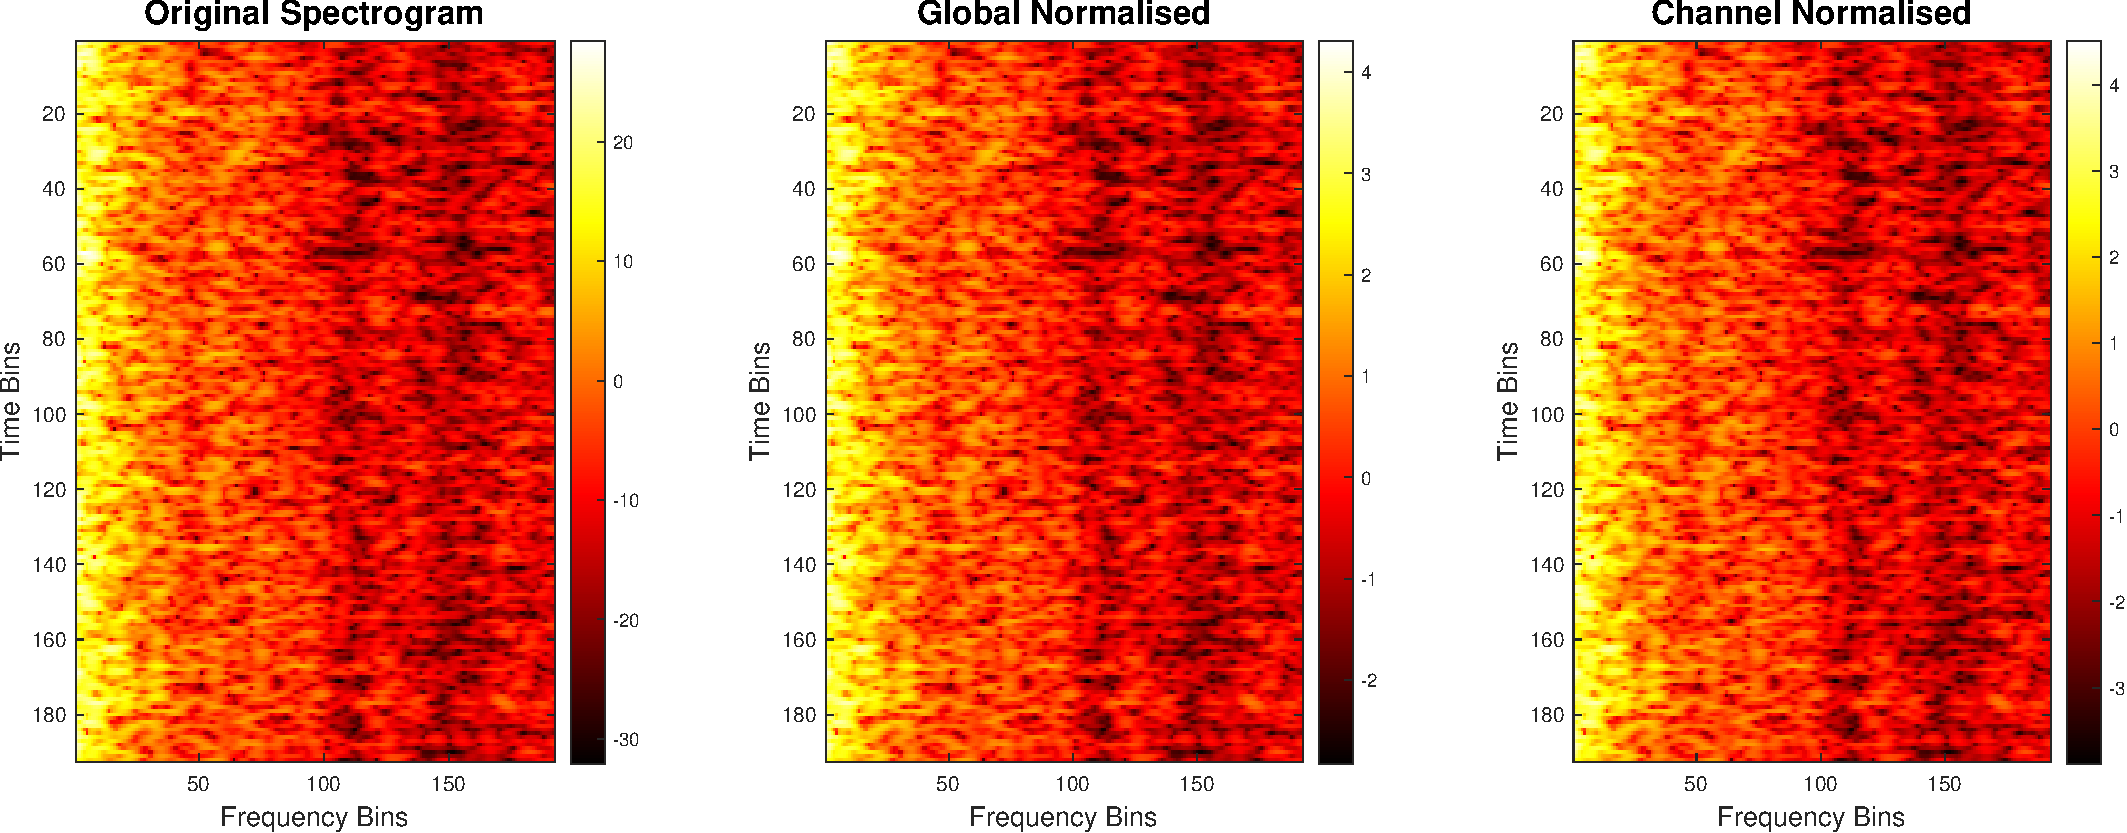
\includegraphics[width=\textwidth]{img/ch4/normalisation/spectrogramComparison.pdf}
        \caption{Comparison of original spectrogram with global-normalised and channel-normalised spectrograms.}
        \label{fig:normalisation-spectrogram}
    \end{subfigure}
    
    \vspace{1cm}
    
    % Subfigure 2: Histogram Comparison
    \begin{subfigure}[t]{\textwidth}
        \centering
        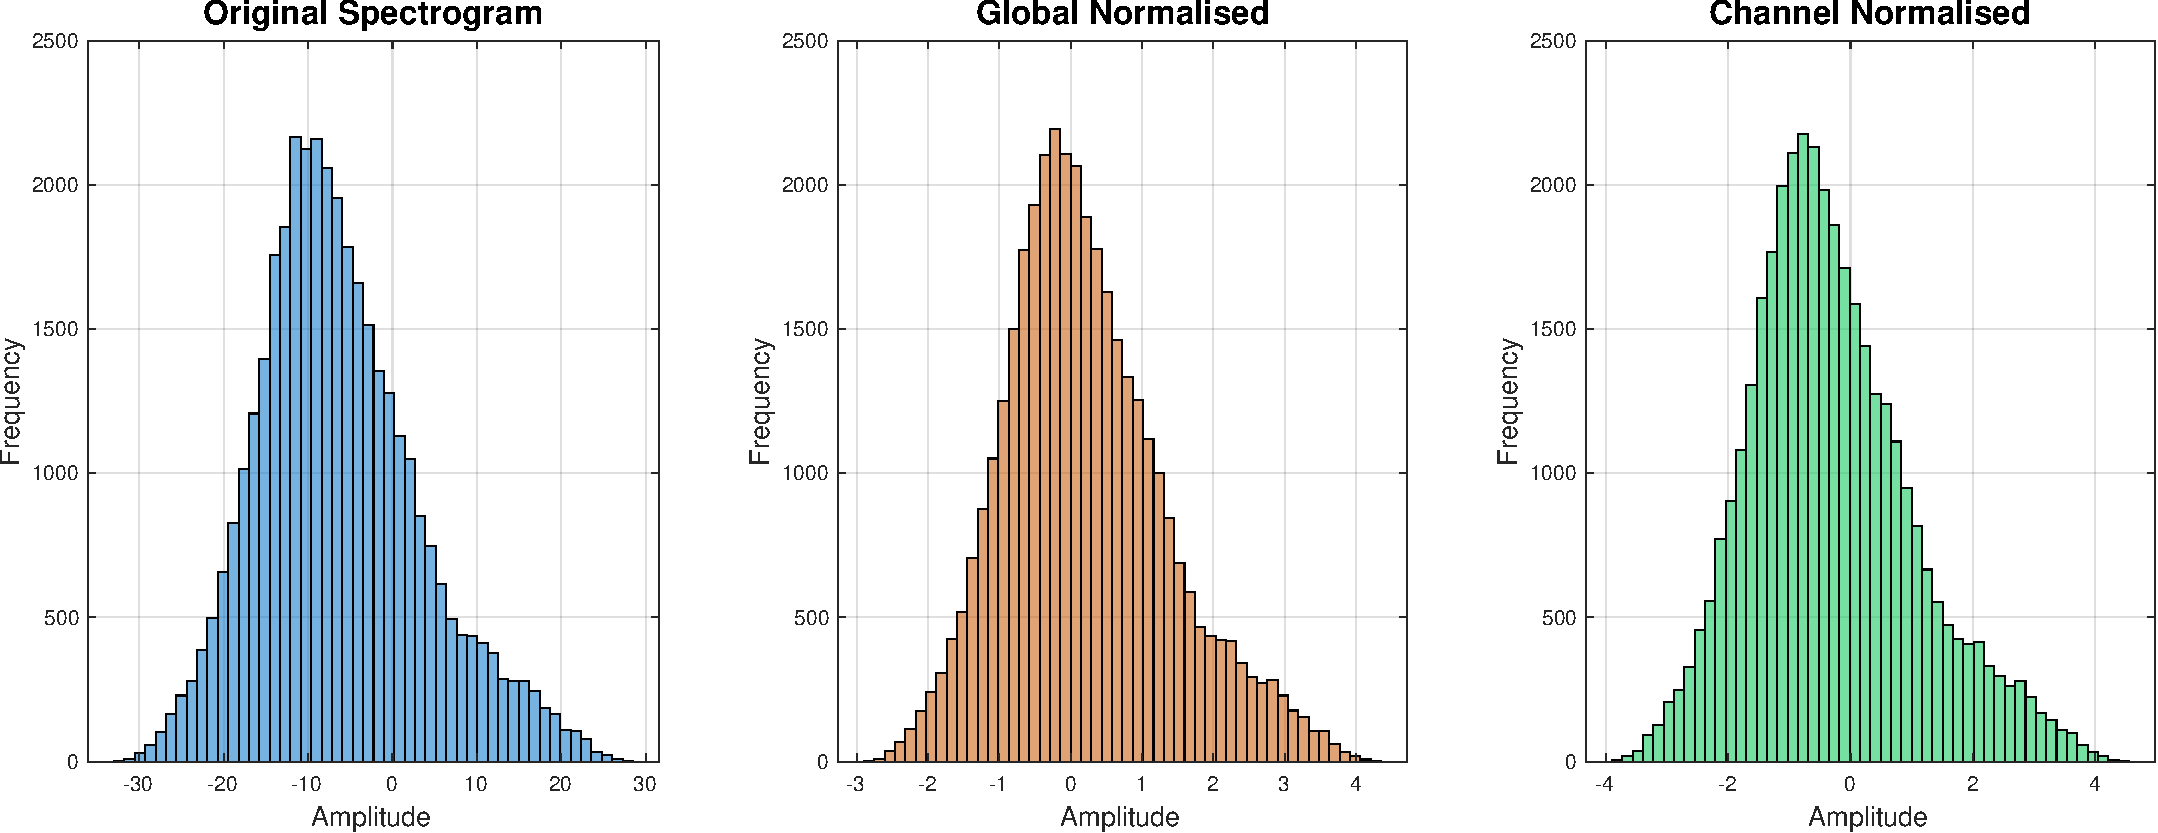
\includegraphics[width=\textwidth]{img/ch4/normalisation/histogramComparison.pdf}
        \caption{Comparison of amplitude histograms for original, global-normalised, and channel-normalised spectrograms.}
        \label{fig:normalisation-histogram}
    \end{subfigure}
    
    \vspace{1cm}
    
    % Subfigure 3: Time Segment Comparison
    \begin{subfigure}[t]{\textwidth}
        \centering
        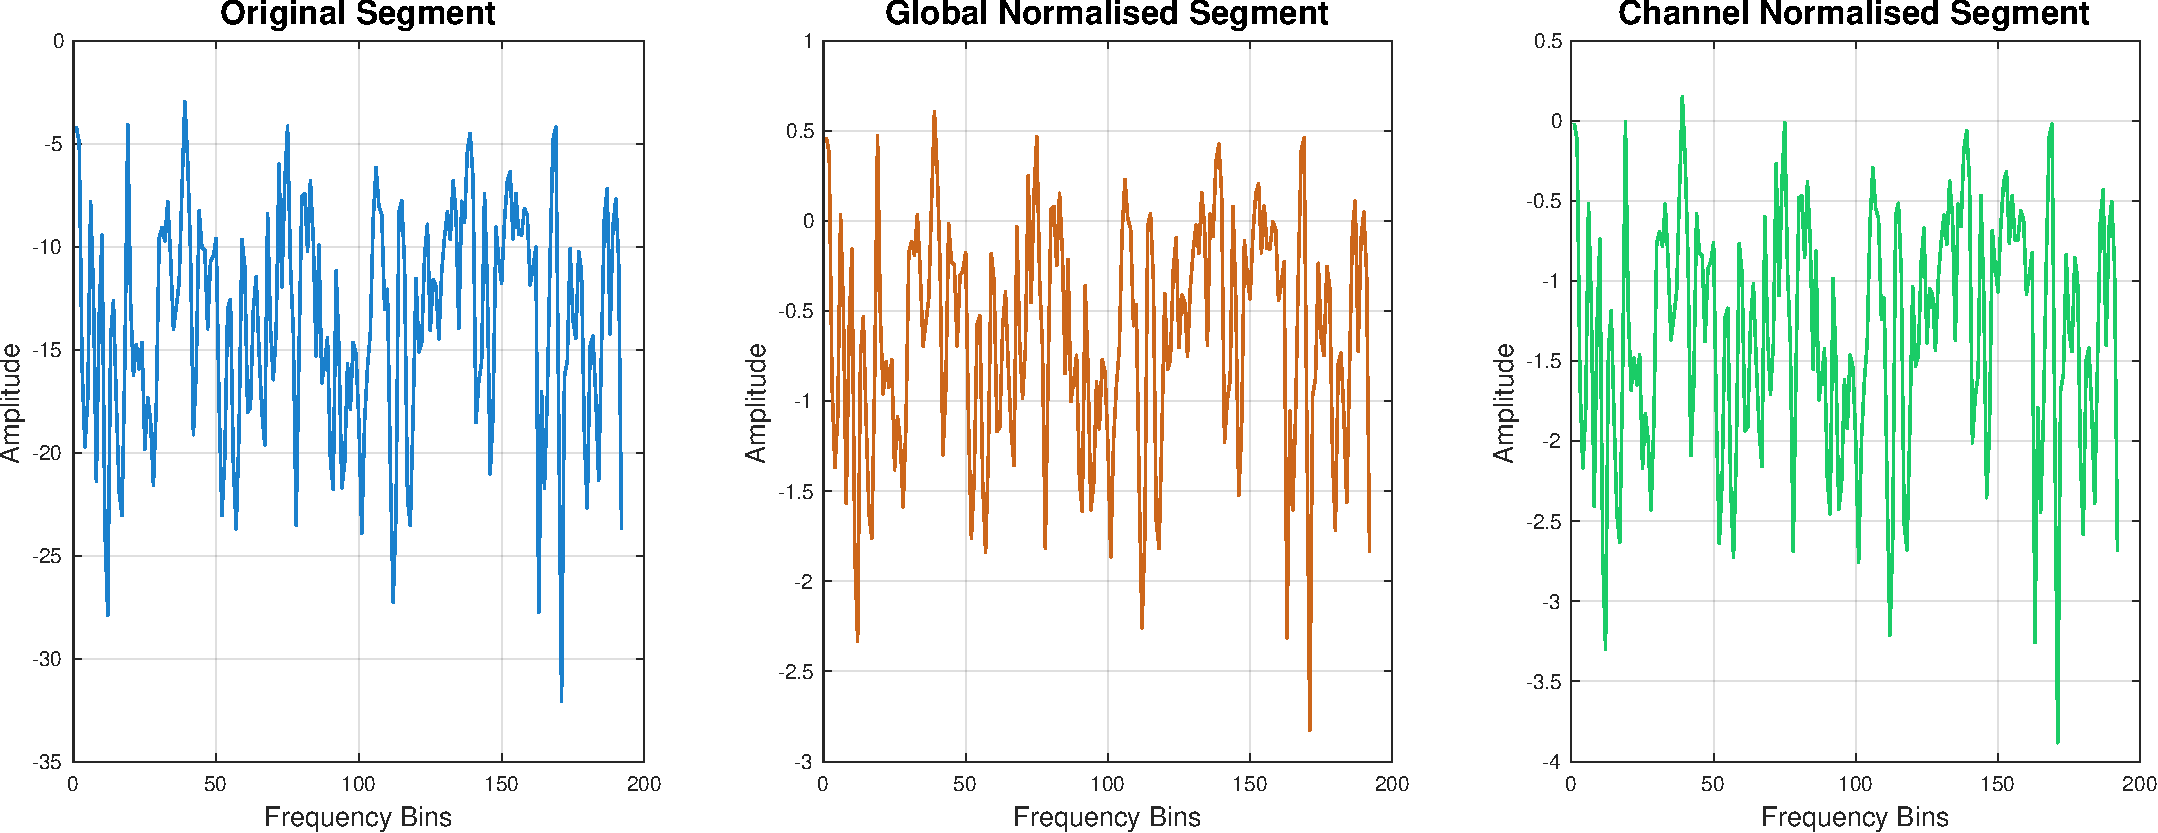
\includegraphics[width=\textwidth]{img/ch4/normalisation/timeSegmentComparison.pdf}
        \caption{Comparison of a random time segment for original, global-normalised, and channel-normalised spectrograms.}
        \label{fig:normalisation-time-segment}
    \end{subfigure}

    \caption{Visual comparison of normalisation methods.}
    \label{fig:normalisation-combined}
\end{figure}

The comparison of original, global-normalised, and channel-normalised spectrograms, as shown in Figure~\ref{fig:normalisation-combined}, reveals minimal visual differences in the structural patterns across the three techniques. This outcome is expected, as the primary purpose of normalisation is not to alter the fundamental features of the spectrogram but to rescale their amplitudes into a standardised range. The key difference in Figure~\ref{fig:normalisation-spectrogram} lies in the colour bar scaling: in the original spectrograms, amplitude values span a range of approximately -30 to 30 dB, whereas in the global and channel-normalised spectrograms, the values are rescaled to a narrower range, approximately -3 to 4 dB. This is further supported by Figure~\ref{fig:normalisation-time-segment} which highlights the rescaling of amplitudes for a single random time segment in each spectrogram. Additionally, the amplitude histograms in Figure~\ref{fig:normalisation-histogram} show that while the overall distribution shapes remain similar, the normalised spectrograms exhibit distributions centred around zero. 

The structural features of the spectrograms remaining unchanged highlights a key property of normalisation: it modifies the scale of the features without altering their spatial or structural characteristics, and consequently, the normalised spectrograms retain the important information necessary for classification while standardising the data for greater gradient stability during machine learning tasks.

\subsubsection{Results and discussion}

The baseline CNN-LSTM model was trained for three epochs on both globally and channel-normalised spectrograms. The input parameters for the model were consistent with those specified in Table~\ref{tab:cnn-lstm-final-params} and the training configuration is the same as that described in Section \ref{subsec:training-configuration}. Table \ref{tab:normalisation-results} summarises the results of the experiment. 

\begin{table}[htbp]
    \centering
    \begin{tabular}{lcc}
        \toprule
        \textbf{Normalisation strategy} & \textbf{Accuracy (\%)} & \textbf{F1-score (\%)} \\
        \midrule
        Baseline (no normalisation)     & 87.94                     & 88.03 \\
        Global normalisation            & 87.15                     & 87.06 \\
        Channel-based normalisation     & 87.98                     & 88.09 \\
        \bottomrule
    \end{tabular}
    \caption{Comparison of normalisation strategies on the DeepShip dataset.}
    \label{tab:normalisation-results}
\end{table}

% \begin{figure}[p]
%     \centering
%     \begin{subfigure}{\textwidth}
%         \centering
%         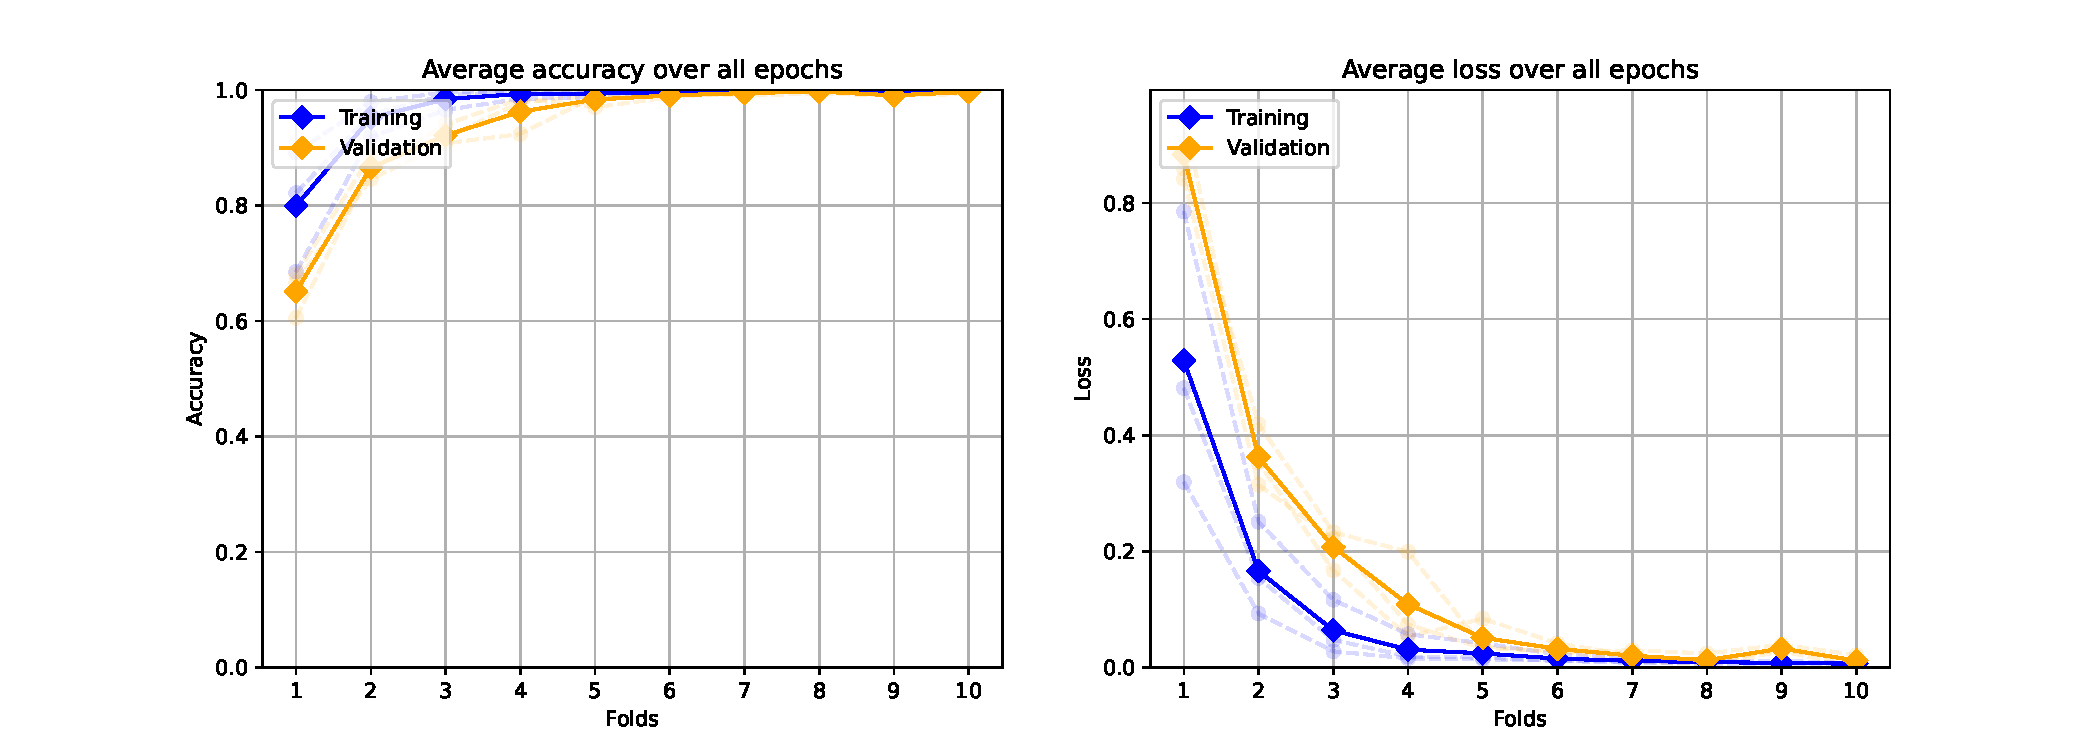
\includegraphics[trim={3cm 0 3cm 0.8cm},clip,width=\textwidth]{img/ch4/normalisation/channel/3_epochs_by_fold.pdf}
%         \caption{}
%         \label{}
%     \end{subfigure}
    
%     \vspace{1cm}
    
%     \begin{subfigure}{\textwidth}
%         \centering
%         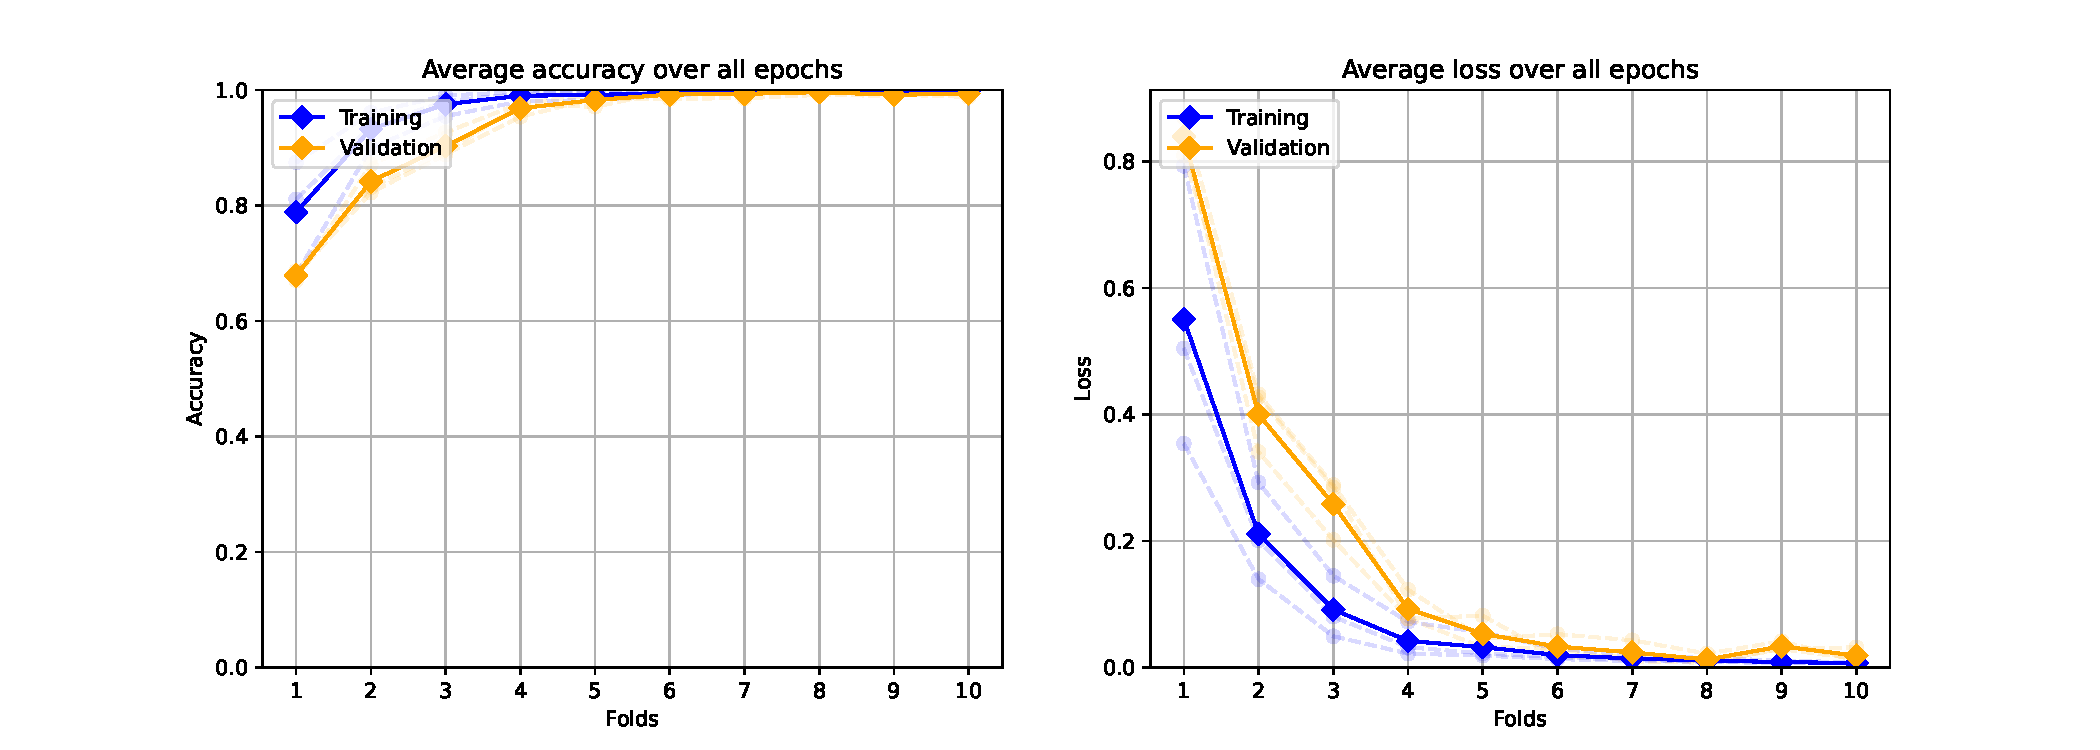
\includegraphics[trim={3cm 0 3cm 0.8cm},clip,width=\textwidth]{img/ch4/normalisation/global/3_epochs_by_fold.pdf}
%         \caption{}
%         \label{}
%     \end{subfigure}
%     \caption{} 
%     \label{}
% \end{figure}

The results of this experiment show minimal difference between the three normalisation strategies. The baseline model achieved an accuracy of 87.94\%, while global normalisation resulted in a slightly lower accuracy of 87.15\%, and channel-based normalisation displayed a marginally higher accuracy of 87.98\%.

This lack of significant improvement was unexpected, particularly given the previous research on the theoretical and practical benefits of normalisation for machine learning tasks \cite{chris_kroenke_normalizing_2022, gunes_answer_2020, wu_group_2018, primus_frequency-wise_2023, simic_normalization_2023}. One possible explanation lies in the relatively consistent scale and distribution of spectrogram features in the DeepShip dataset. Unlike datasets where input features vary drastically, the spectrograms in this dataset may already have a well-balanced scale, reducing the need for aggressive normalisation. Furthermore, the logarithmic transformation undertaken to convert the spectrogram into its power representation likely already contributed to standardising the input values to some extent, minimising the impact of explicit normalisation techniques.

A key limitation of the experiment was the approach taken to calculate the normalisation statistics. In standard practice, the mean and standard deviation are calculated on the training set and then applied to both the training and test sets. This ensures that the test data remains unseen during the calculation of normalisation parameters, preserving the integrity of the evaluation process and preventing data leakage. However, due to the $k$-fold cross-validation setup used in this study, where training and testing sets change dynamically in each fold, it was impractical to calculate the mean and standard deviation exclusively from the training set. Instead, normalisation statistics were computed using the entire dataset, which may have introduced a minor data leakage effect. While this compromise was necessary given the experimental constraints, it could explain the minimal differences observed between the strategies.

Additionally, it is possible that the relatively short training duration of three epochs limited the ability of the model to fully leverage any benefits introduced by normalisation. Normalisation's primary advantages, such as stabilising gradient flow and accelerating convergence, may become more evident over longer training periods or with deeper models.

Finally, it is worth noting that while normalisation did not significantly impact classification accuracy, it may still have other advantages not captured in this experiment, such as enabling more efficient training and model convergence. Future work could explore these aspects more thoroughly.

In conclusion, this experiment did not reveal a substantial impact of normalisation on classification metrics for the DeepShip dataset. This highlights the importance of taking into account dataset characteristics when designing and implementing preprocessing techniques. Further investigations into alternative normalisation approaches or a time-based comparison of normalisation techniques may provide deeper insights into the role of normalisation in UATR tasks.

%%%%%%%%%%%%%%%%%%%%%%%%%%%%%%%%%%%%%%%%%%%%%%%%%%%%%%%%%%%%%%%
\section{Detrending}

Detrending is the process of removing long-term trends from data to focus on irregular fluctuations and periodic signals that may be more informative for analysis. In the context of audio spectrograms, detrending separates the underlying noise from the desired signals, allowing the periodicity of narrowband events to become more prominent. Unlike smoothing, which reduces noise to clarify long-term trends, detrending eliminates these trends to better reveal short-term patterns and fluctuations.

The motivation for exploring detrending in this thesis is twofold. First, in UATR classification tasks, detrending can suppress underlying broadband noise that may obscure key acoustic features, such as the periodic sounds generated by ship propellers. By isolating these high-frequency components, detrended spectrograms can serve as more effective inputs for machine learning models, potentially improving classification performance. Second, detrended spectrograms may visually enhance narrowband events, such as ship-radiated noise segments, making them more suitable for image segmentation tasks. This could facilitate the manual training of feature extraction models or enable clearer identification of specific signal features for downstream analysis. The focus of this thesis is therefore to evaluate the effectiveness of detrending in both these applications, particularly using the $\ell_1$ detrending algorithm to process spectrograms for improved signal clarity and classification utility.

\subsection{Overview of detrending algorithms}

Detrending algorithms aim to remove underlying trends from data, isolating the fluctuations that are more relevant for analysis. Mathematically, we can describe this as idea as an optimisation problem. We are given a scalar time series $y_t$, $t = 1, \ldots, n$, assumed to consist of an underlying slowly varying trend $x_t$, and a more rapidly varying random component $z_t$. Our goal is to estimate the trend component $x_t$, or equivalently, estimate the random component $z_t = y_t - x_t$. 

This section provides an overview of commonly used methods and introduces the $\ell_1$ detrending algorithm, which is the focus of this section.

\subsubsection{Differencing}
The simplest detrending method involves differencing the data. For a dataset with points $(x_1, x_2, \ldots, x_n)$, detrending by differencing computes a new dataset as $(x_2 - x_1, x_3 - x_2, \ldots, x_n - x_{n-1})$. While straightforward, this method can be overly sensitive to noise, as it does not distinguish between the trend and high-frequency fluctuations.

\subsubsection{Model fitting}
Another widely used approach is to detrend by fitting a model to the data and removing the fitted trend. A simple example is linear detrending, where a line is fit to the data via least squares regression, and the residuals (differences between observed and predicted values) make up the detrended result. More complex versions of this technique involve fitting higher-order polynomials or other parametric models to capture nonlinear trends. While effective, these methods require assumptions about the nature of the trend and can be prone to overfitting if the model is too complex.

\subsubsection{Hodrick-Prescott filter}
The Hodrick-Prescott (H-P) filter is a widely used detrending technique in time-series analysis, particularly in economics \cite{hodrick_postwar_1997}. It decomposes a signal into a trend component and a cyclical component by solving an optimisation problem that minimises a loss function combining two competing objectives: the closeness of the trend to the data and the smoothness of the trend. Specifically, the H-P filter minimises:
\begin{equation}
    \sum_{t=1}^n (y_t - x_t)^2 + \lambda \sum_{t=2}^{n-1} (x_{t-1} - 2x_t + x_{t+1})^2
\end{equation}
where $y_t$ is the observed signal, $x_t$ is the trend, and $\lambda$ is the smoothing parameter. The first term enforces the trend's closeness to the original data, while the second term penalises sharp changes in the trend to ensure smoothness.

The smoothing parameter $\lambda$ plays a crucial role: larger $\lambda$ values result in smoother trends, while smaller $\lambda$ values retain more of the original signal's variability. While the H-P filter is effective for detecting long-term trends in economic data, it has limitations. It assumes that the trend is smooth, making it less effective for signals with sharp changes or localised features. Additionally, its reliance on the $\ell_2$ norm in the smoothness term can make it sensitive to outliers, which disproportionately affect the squared differences.

\subsubsection{\texorpdfstring{$\ell_1$}{l1} Detrending Algorithm}
The $\ell_1$ detrending algorithm \cite{kim_ell_1_2009} builds on the principles of the H-P filter but replaces the $\ell_2$ norm in the smoothness penalty with the $\ell_1$ norm. This modification makes the $\ell_1$ algorithm more robust to outliers and better suited to capturing sharp changes in the trend. The optimisation problem for $\ell_1$ detrending is expressed as:
\begin{equation}
    \frac{1}{2} \sum_{t=1}^n (y_t - x_t)^2 + \lambda \sum_{t=2}^{n-1} \| x_{t-1} - 2x_t + x_{t+1} \|
\end{equation}
Here, the $\ell_1$ norm ($\| \cdot \|$) in the second term penalises large differences between successive points in the trend, enforcing smoothness while preserving sharp transitions.

The $\ell_1$ detrending algorithm retains the flexibility of the H-P filter with its tunable regularisation parameter $\lambda$, but its use of the $\ell_1$ norm allows it to better handle datasets with localised events or abrupt changes. Ship radiated noise, for instance, often contains periodic narrowband features from machinery noise, which can be masked by the broadband components in the signal. The $\ell_1$ algorithm’s sensitivity to these features makes it particularly suitable for UATR tasks. By fine-tuning $\lambda$, we can strike a balance between removing the trend and preserving the narrowband features critical for both classification and visual analysis.

\subsection{Implementation}

The $\ell_1$ detrending algorithm was implemented in MATLAB as a modular and flexible function which builds upon the original code published by the authors. The primary objective of this implementation was to enable experimentation with different detrending strengths through tweaking the regularisation parameter $\lambda$, which we assign a coefficient $\alpha$, as well as provide visualisations to evaluate the effectiveness of detrending for classification and image segmentation tasks.

The detrending algorithm is formulated as an optimisation problem where we try to balance two objectives: minimising the residual between the input signal and its estimated trend while ensuring that the trend remains smooth. The regularisation parameter $\lambda$ governs this trade-off. For any given signal, $\lambda_{\text{max}}$ is the value of $\lambda$ beyond which the algorithm will simply return a 1-to-1 translation, or \textit{affine fit}, for the data. This upper bound is computed using a function provided by the authors, \texttt{l1tf\_lambdamax}. The value of $\lambda$ used during detrending is then defined as a fraction of $\lambda_{\text{max}}$, controlled by the coefficient $\alpha$. By experimenting with various values of $\alpha$, it is possible to fine-tune the balance between trend smoothness and residual suppression.

\begin{figure}[htbp]
    \centering
    % Subfigure 1: Segment trend plot
    \begin{subfigure}[t]{\textwidth}
        \centering
        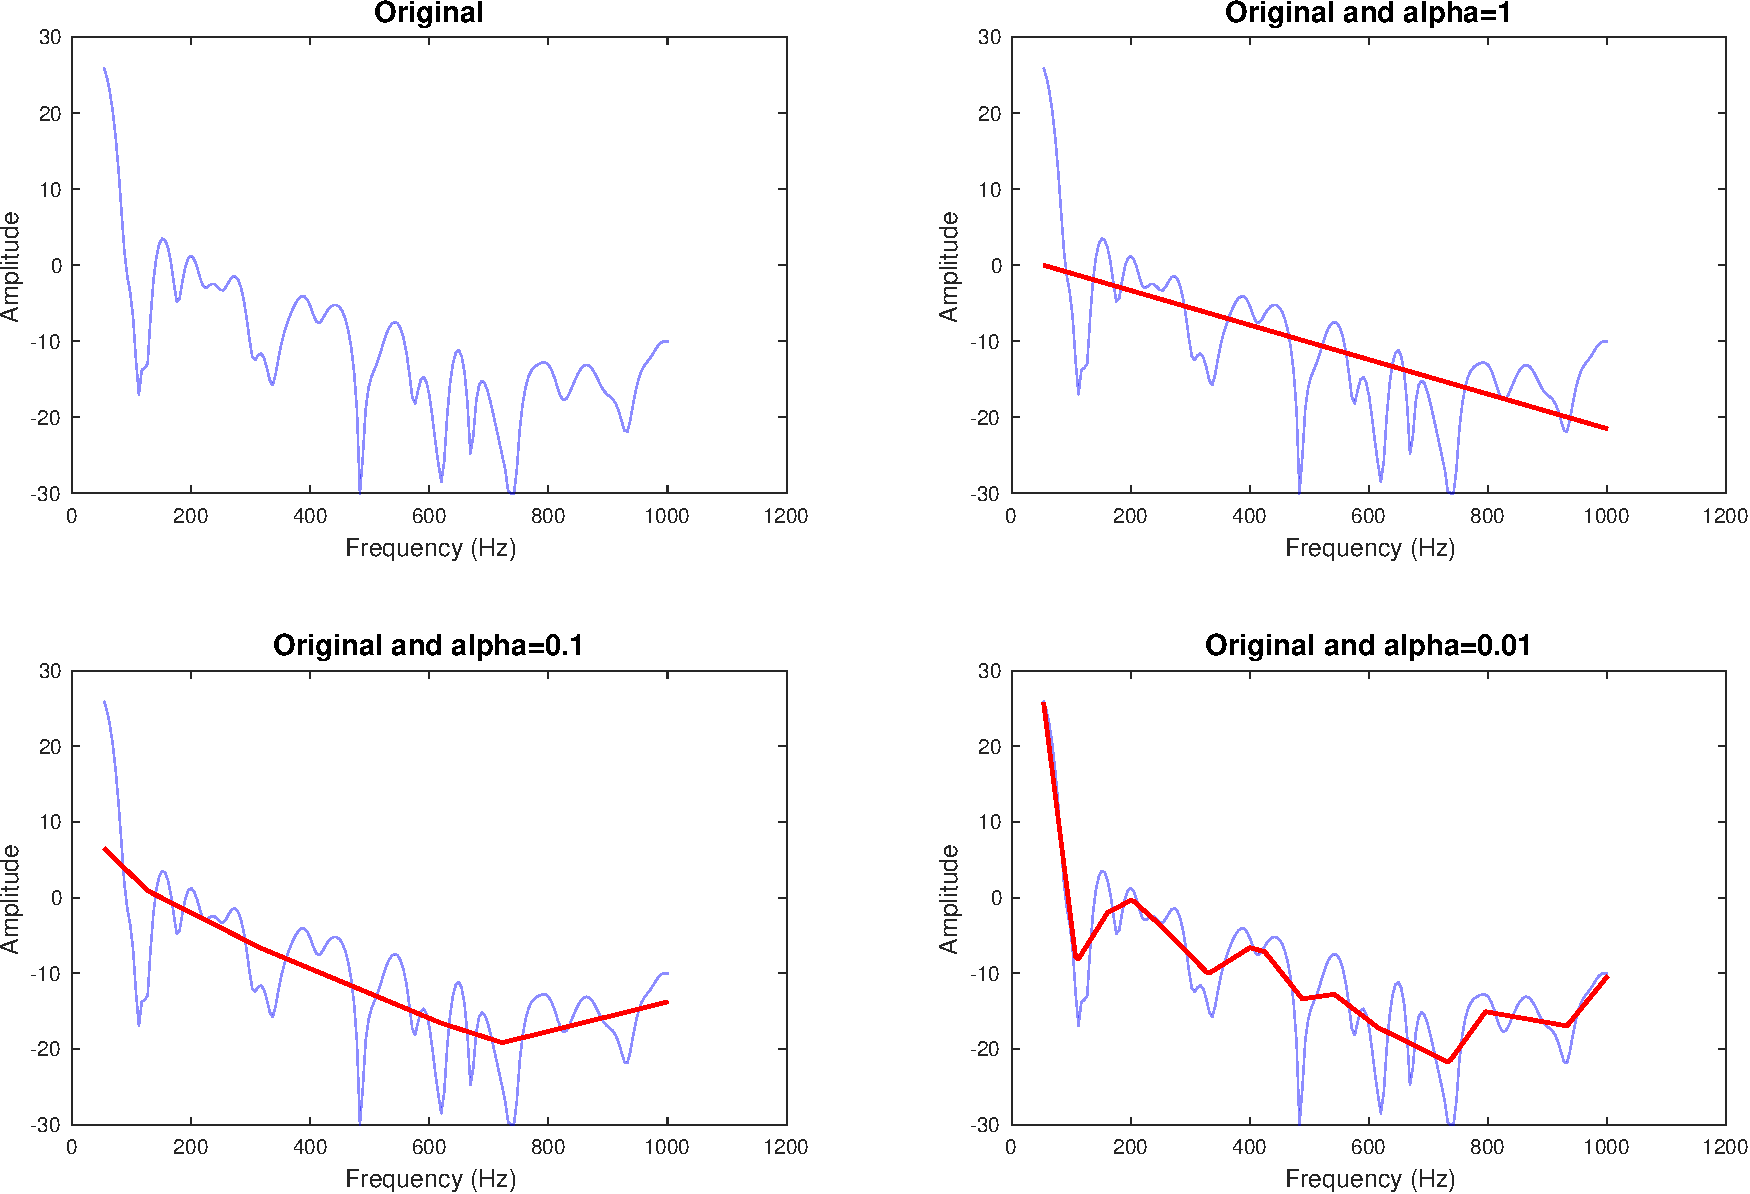
\includegraphics[width=\textwidth]{img/ch4/l1/example_l1_plots/segment_l1_trend.pdf}
        \caption{Overlay of a random time segment with its corresponding $\ell_1$ trend at various $\alpha$ values.}
        \label{fig:l1:segment-trend}
    \end{subfigure}
    
    \vspace{1cm}
    
    % Subfigure 2: Segment detrended plot
    \begin{subfigure}[t]{\textwidth}
        \centering
        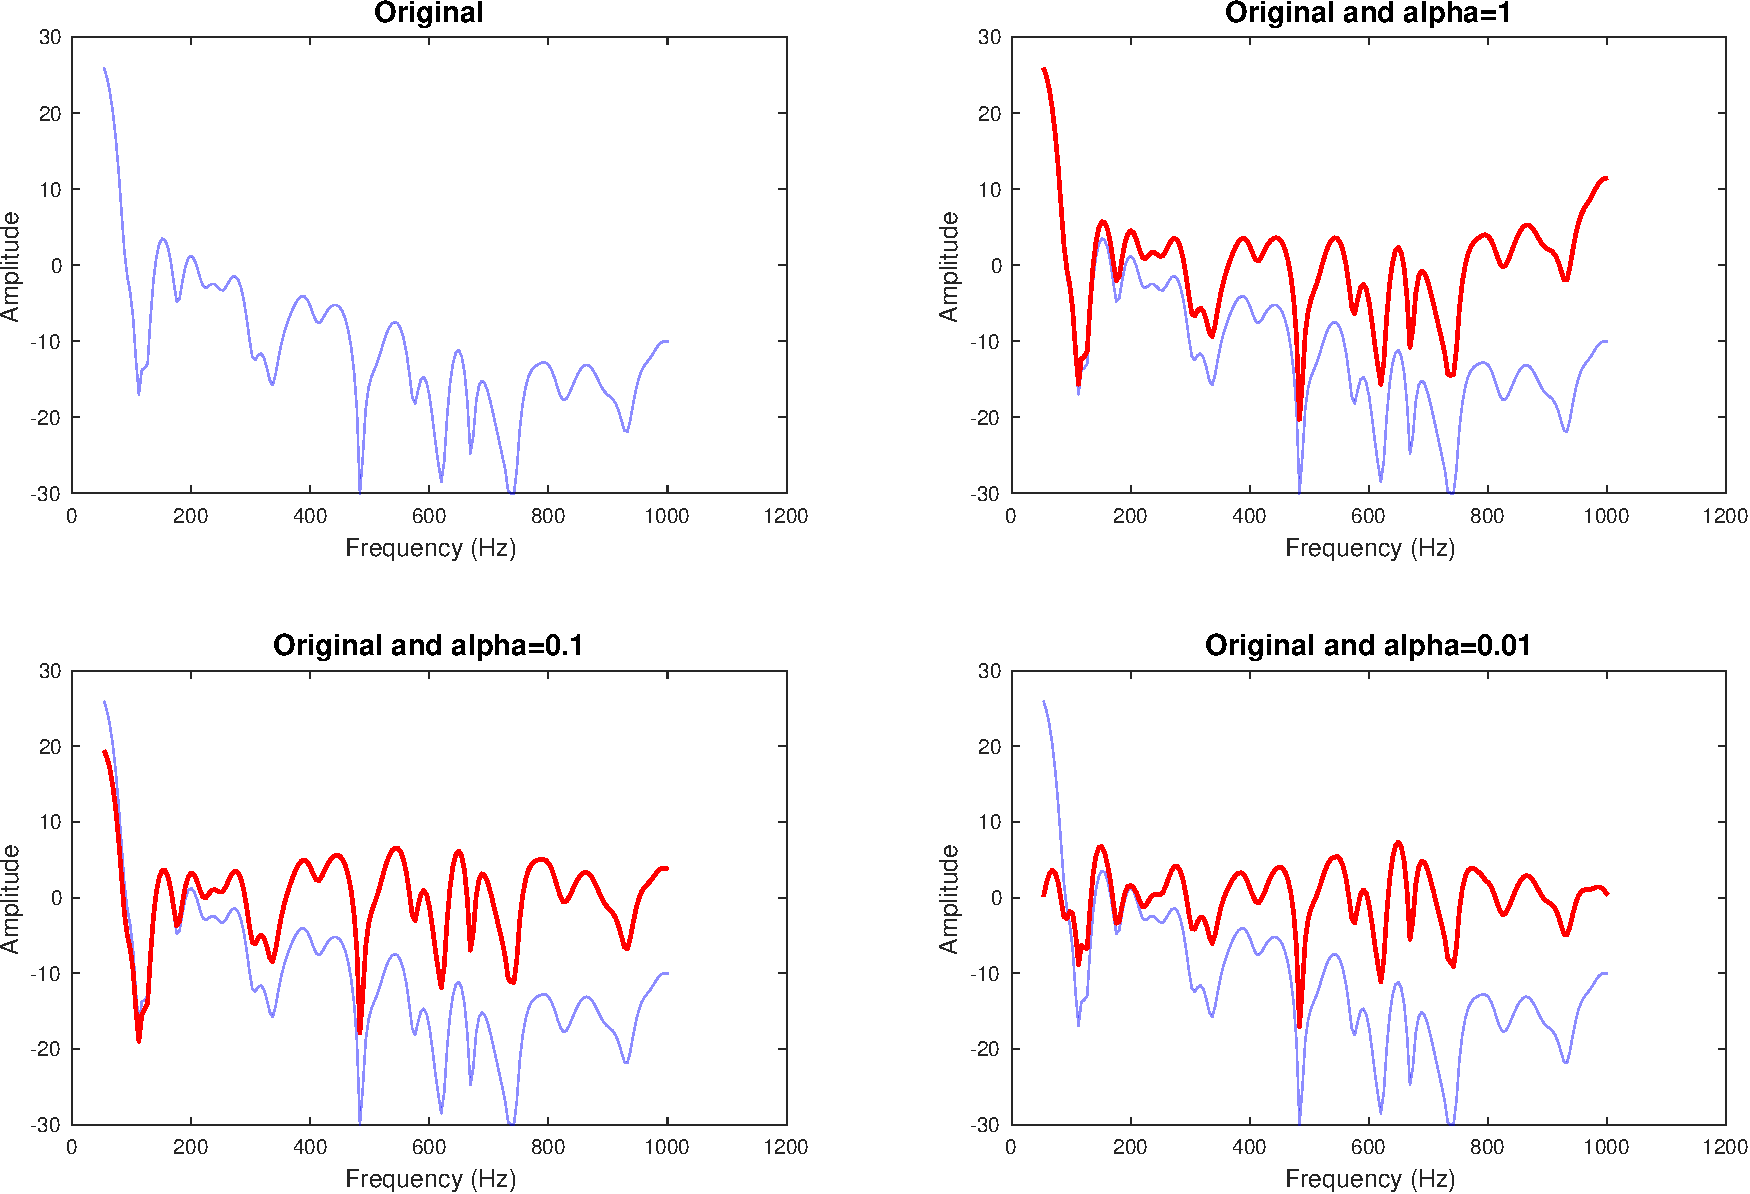
\includegraphics[width=\textwidth]{img/ch4/l1/example_l1_plots/segment_detrended.pdf}
        \caption{Random time segment before and after detrending at different $\alpha$ values, highlighting the removal of long-term trends in the signal.}
        \label{fig:l1:segment-detrended}
    \end{subfigure}
\end{figure}

\begin{figure}
    \ContinuedFloat
    % Subfigure 3: Spectrogram comparison
    \begin{subfigure}[t]{\textwidth}
        \centering
        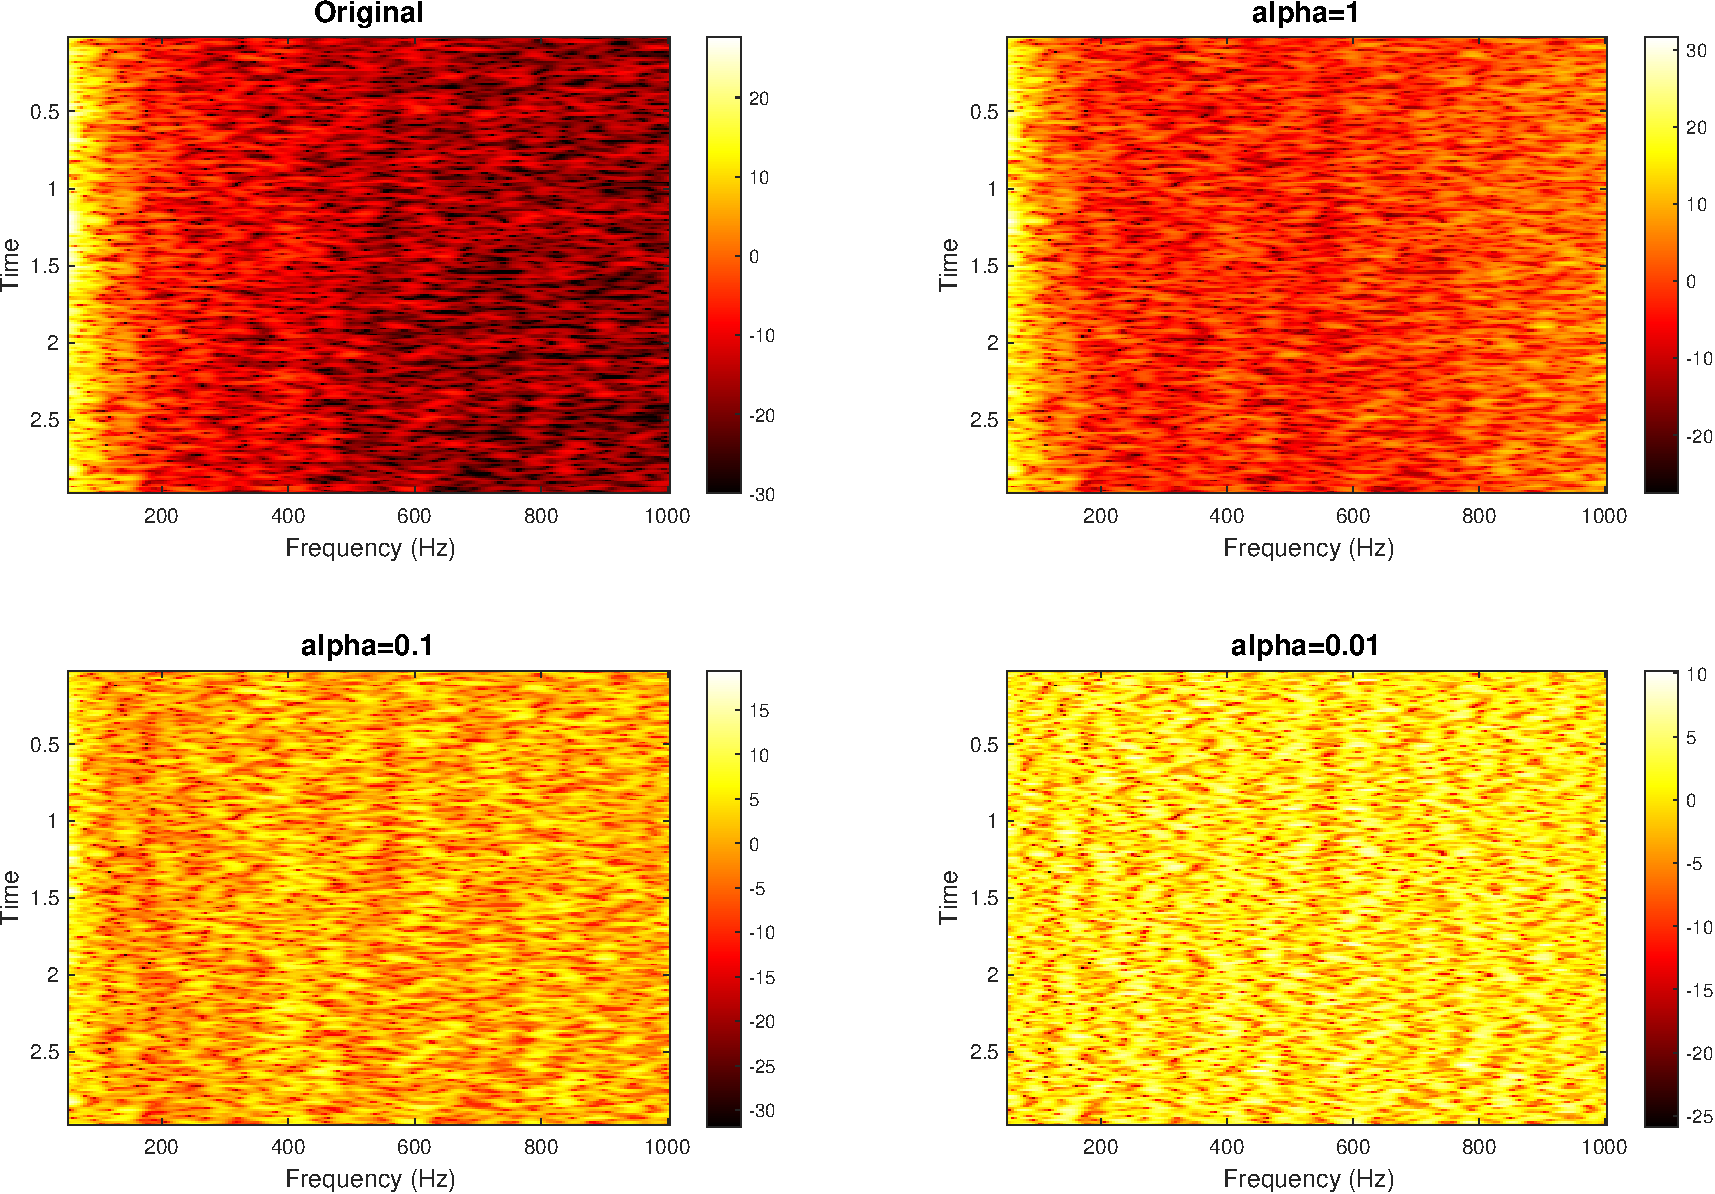
\includegraphics[width=0.95\textwidth]{img/ch4/l1/example_l1_plots/spec_comparison.pdf}
        \caption{Comparison of original and detrended spectrograms produced using $\ell_1$ detrending at various $\alpha$ values.}
        \label{fig:l1:spectrogram-comparison}
    \end{subfigure}
    
    \vspace{1cm}
    
    % Subfigure 4: 3D surface plots
    \begin{subfigure}[t]{\textwidth}
        \centering
        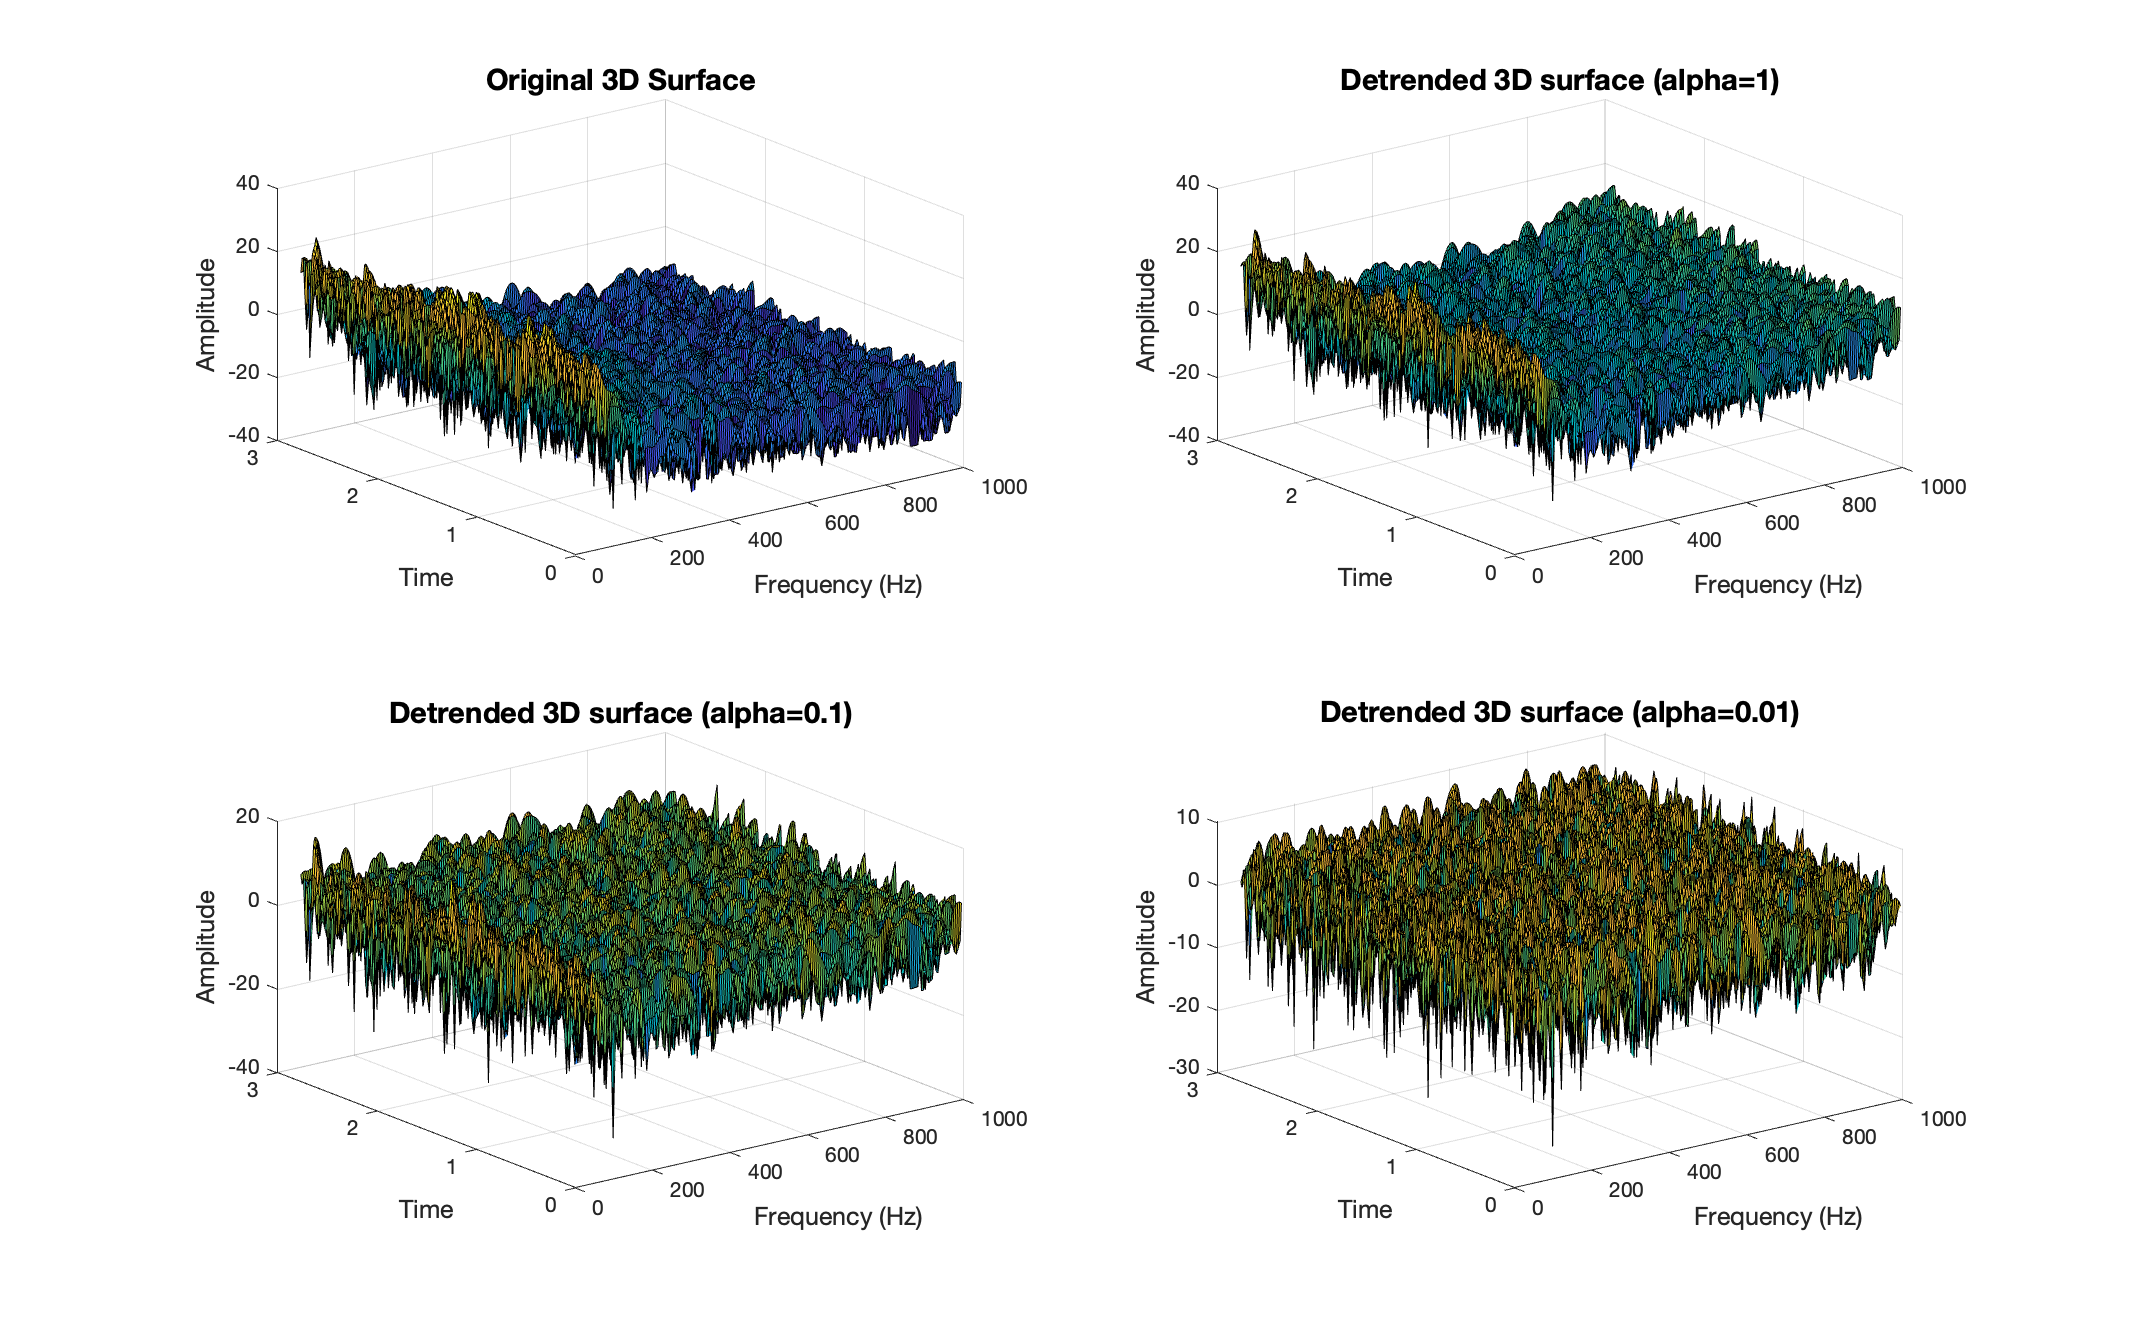
\includegraphics[trim={3cm 1.5cm 2.5cm 1cm},clip,width=0.95\textwidth]{img/ch4/l1/example_l1_plots/3d_plot.pdf} %{left bottom right top}
        \caption{Three-dimensional surface plots of the original spectrogram and detrended spectrograms at different $\alpha$ values.}
        \label{fig:l1:3d}
    \end{subfigure}
    \caption{Visual analysis of $\ell_1$ detrending for various $\alpha$ values, illustrating its impact on spectrograms through comparative visualisations, time-segment overlays, and 3D surface plots.}
    \label{fig:l1:overview}
\end{figure}

To support this experimentation, our implementation of the $\ell_1$ detrending algorithm allows the user to specify up to 10 values of $\alpha$ in a single run. The function computes detrended spectrograms for each specified $\alpha$ value and generates a range of diagnostic plots that facilitate analysis. These visualisations were incredibly helpful in helping select appropriate values for $\alpha$ for subsequent experiments:
\begin{itemize}
    \item Segment trend plot: This plot (Figure~\ref{fig:l1:segment-trend}) overlays a single random time segment with its corresponding $\ell_1$ trends for various $\alpha$ values. By examining the degree of smoothing introduced for different $\alpha$, we could evaluate how effectively the algorithm removed noise without discarding important signal features. Smaller $\alpha$ values were observed to retain more signal detail but were less effective at suppressing noise, while larger $\alpha$ values removed noise more aggressively but often smoothed out transient features.
    \item Segment detrended plot: This diagnostic (Figure~\ref{fig:l1:segment-detrended}) shows the same time segment before and after detrending for various $\alpha$ values. It is the most helpful diagnostic plot to visualise the changes introduced by detrending, especially the removal of long-term trends such as those created by background noise.
    \item Spectrogram comparison: This diagnostic plot (Figure~\ref{fig:l1:spectrogram-comparison}) presents the original spectrogram alongside detrended spectrograms generated using different $\alpha$ values. It provides an overview of how detrending affects the overall amplitude structure, particularly in regions dominated by long-term trends or broadband noise. By visually assessing these plots, we could identify the boundaries where detrending was either too aggressive (overfitting) or too weak (underfitting).
    \item 3D surface plots: These 3D plots provide an alternative representation of how detrending impacts amplitude values across time and frequency (Figure \ref{fig:l1:3d}).
\end{itemize}

Using these diagnostic plots, we determined that $\alpha$ values in the range $[10^{-3}, 1]$ provided a suitable balance between noise suppression and signal preservation. Hence, we chose three such $\alpha$ values for further experimentation: $10^{-2}$, $10^{-1},$ and $1$. These values were chosen in hopes of capturing a wide spectrum of detrending strengths, ranging from subtle noise suppression to more aggressive trend removal.

\subsection{Experiments}

To evaluate the effect of $\ell_1$ detrending on UATR classification performance, the baseline 3-second DeepShip spectrograms (Section \ref{sec:inputs}) were processed using the three selected $\alpha$ values ($10^{-2}$, $10^{-1},$ and $1$). Each detrended spectrogram was saved to a separate directory as a \texttt{.mat} file and subsequently used as input to the CNN-LSTM baseline model. The results, compared to the baseline model trained on non-detrended spectrograms, are presented in Table \ref{tab:detrend-results-3s}.

\begin{table}[htbp]
    \centering
    \begin{tabular}{lcc}
        \toprule
        \textbf{Detrending parameter} & \textbf{Accuracy (\%)} & \textbf{F1-score (\%)} \\ \midrule
        Baseline (no detrending)      & 87.94 & 88.03 \\
        $\alpha = 10^{-2}$            & 81.45 & 81.28 \\
        $\alpha = 10^{-1}$            & 78.70 & 78.89 \\
        $\alpha = 1$                  & 81.45 & 80.76 \\
        \bottomrule
    \end{tabular}
    \caption{Classification results using $\ell_1$ detrending algorithm at various $\alpha$.}
    \label{tab:detrend-results-3s}
\end{table}

\begin{figure}[p]
    \centering
    \begin{subfigure}{\textwidth}
        \centering
        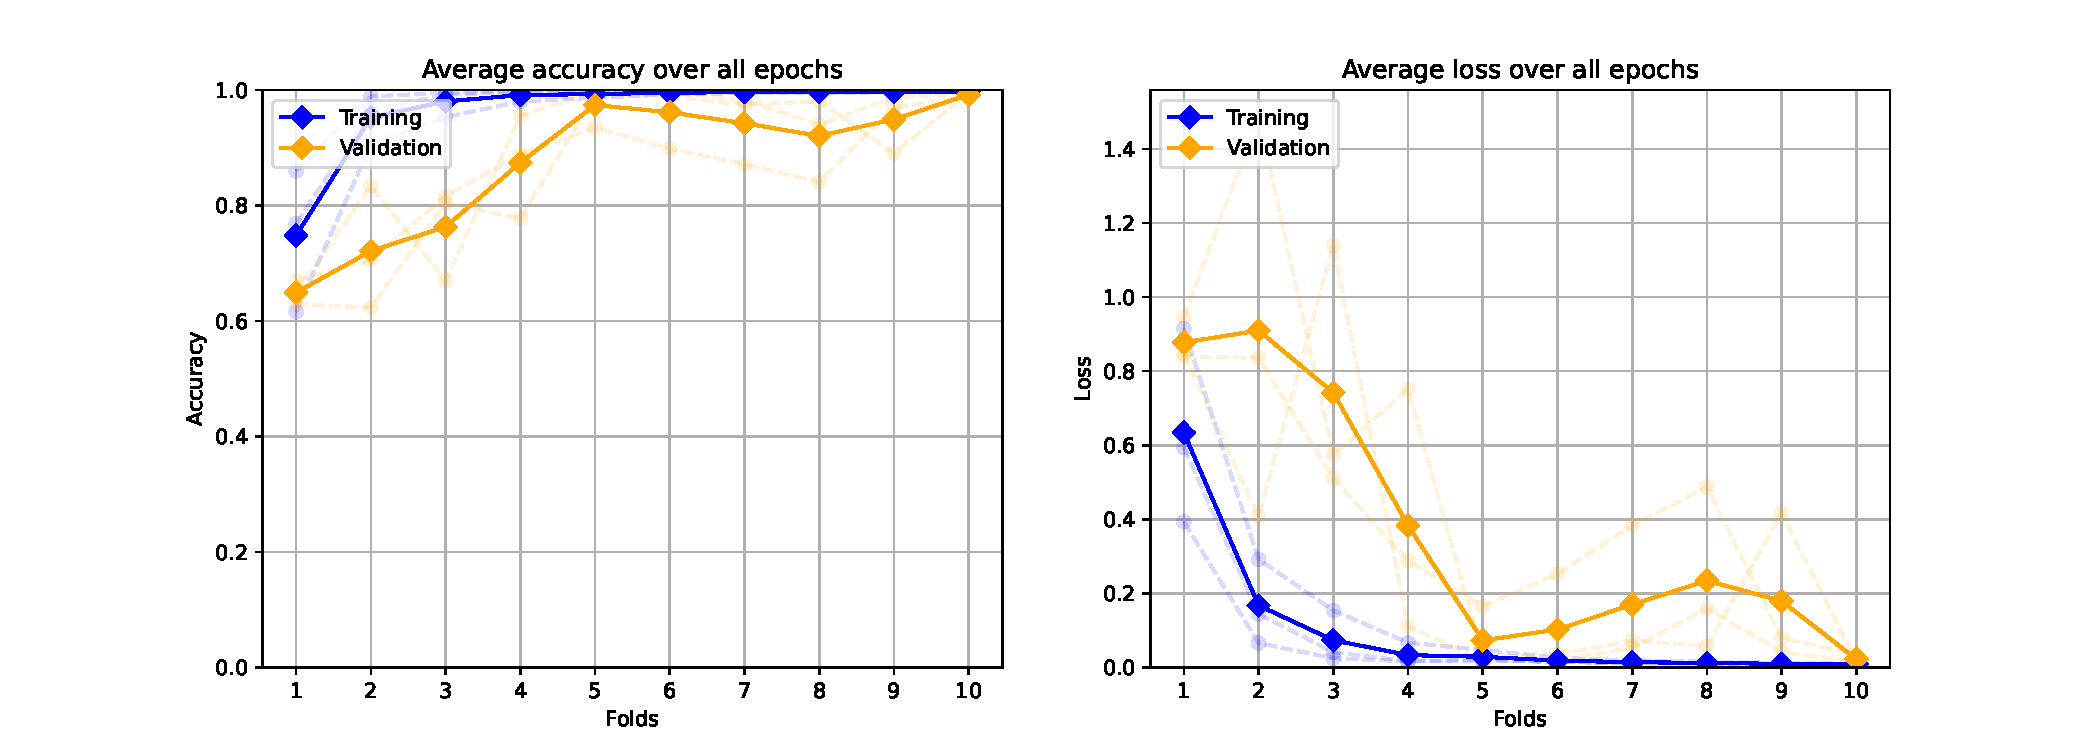
\includegraphics[trim={3cm 0 3cm 0.8cm},clip,width=\textwidth]{img/ch4/l1/e0/3_epochs_by_fold.pdf}
        \caption{Validation accuracy and loss by epoch for $\ell_1$ detrending with $\alpha = 1$.}
        \label{fig:detrend-acc-loss-3s-e-0}
    \end{subfigure}

    \vspace{0.5cm}
    
    \begin{subfigure}{\textwidth}
        \centering
        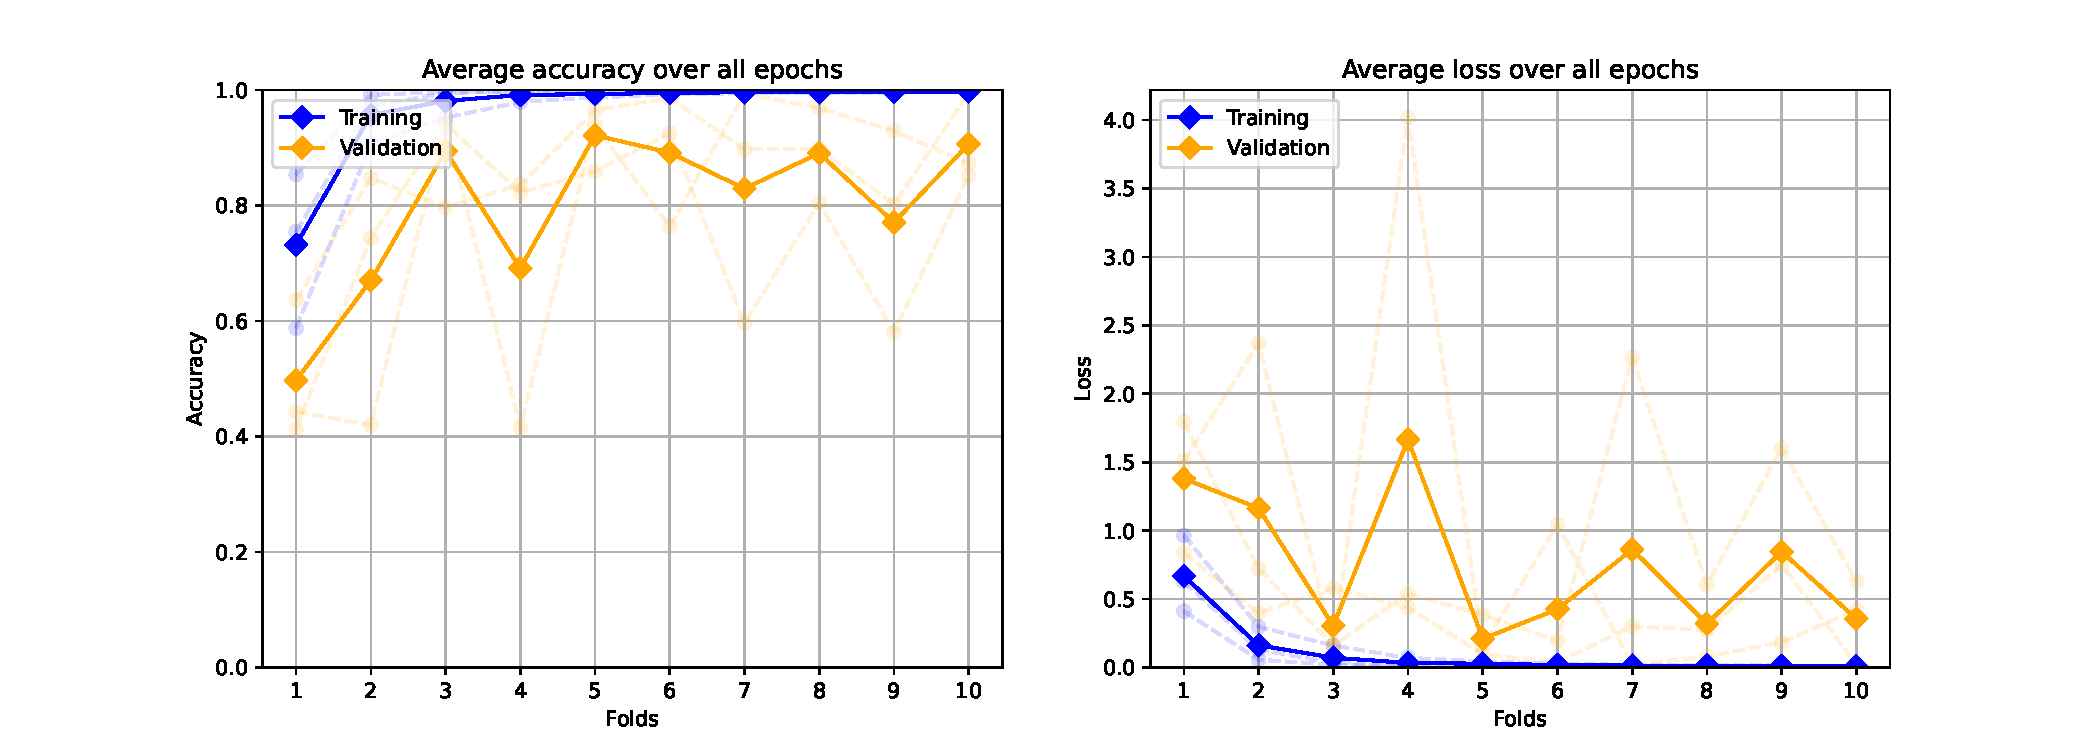
\includegraphics[trim={3cm 0 3cm 0.8cm},clip,width=\textwidth]{img/ch4/l1/e-1/3_epochs_by_fold.pdf}
        \caption{Validation accuracy and loss by epoch for $\ell_1$ detrending with $\alpha = 10^{-1}$.}
        \label{fig:detrend-acc-loss-3s-e-1}
    \end{subfigure}

    \vspace{0.5cm}
    
    \begin{subfigure}{\textwidth}
        \centering
        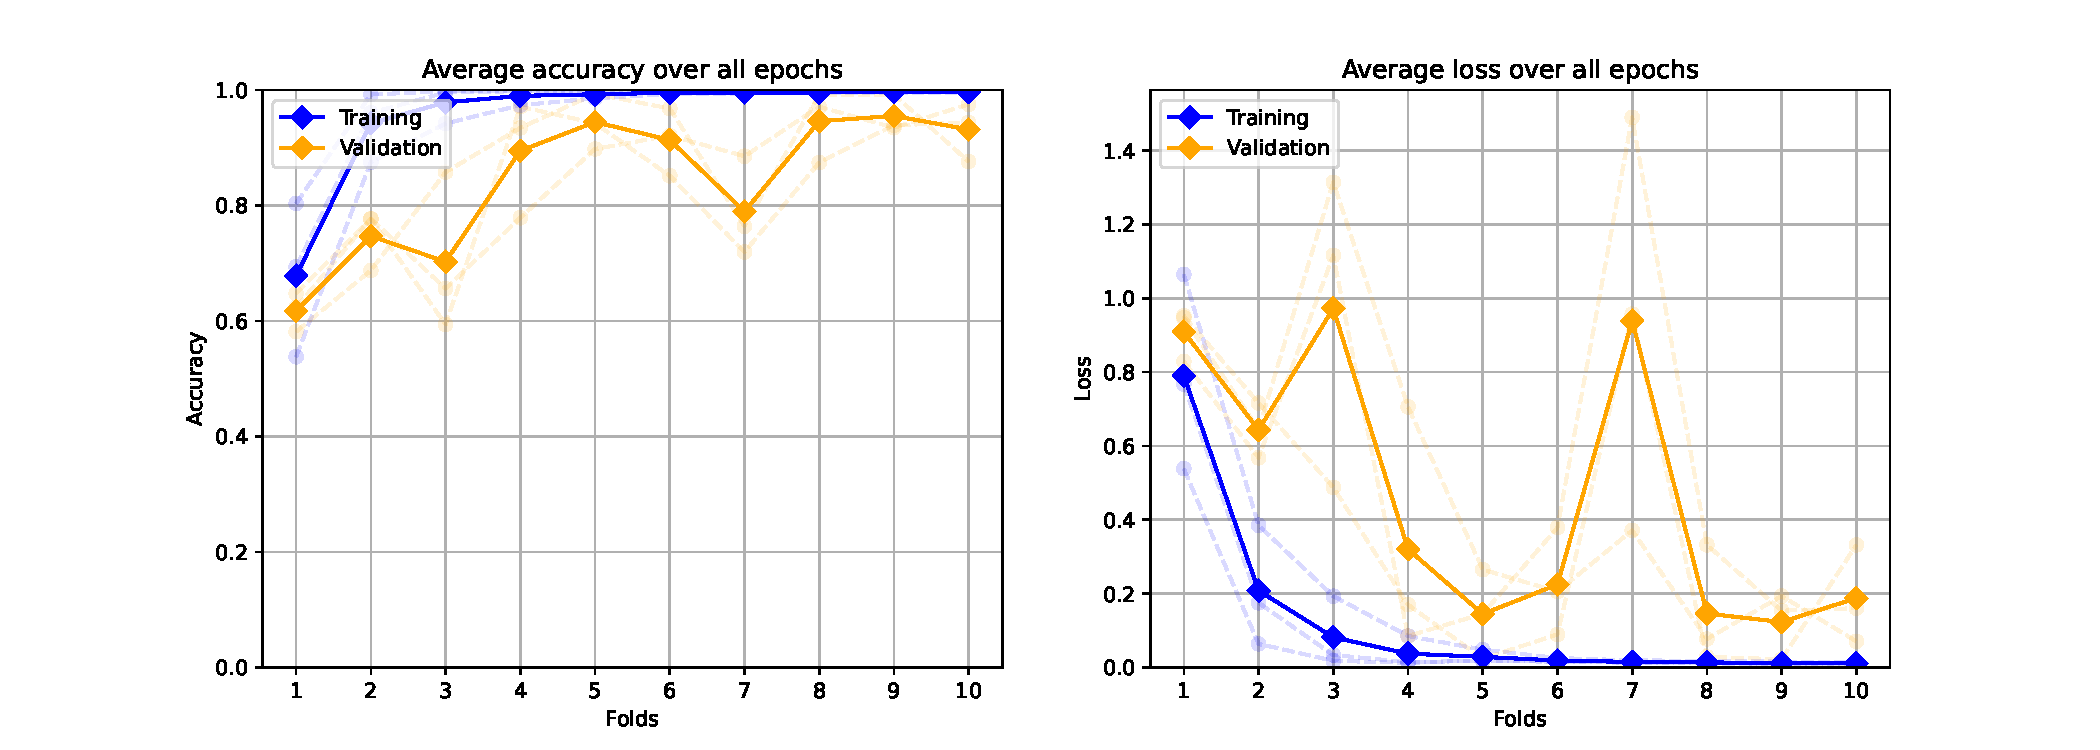
\includegraphics[trim={3cm 0 3cm 0.8cm},clip,width=\textwidth]{img/ch4/l1/e-2/3_epochs_by_fold.pdf}
        \caption{Validation accuracy and loss by epoch for $\ell_1$ detrending with $\alpha = 10^{-2}$.}
        \label{fig:detrend-acc-loss-3s-e-2}
    \end{subfigure}
    \caption{Validation accuracy and loss curves.}    
    \label{fig:detrend-acc-loss-curves-3s}
\end{figure}

The results are quite underwhelming. Table \ref{tab:detrend-results-3s} shows that all three selected $\alpha$ values produced significantly lower classification accuracies and F1-scores compared to the baseline model trained on non-detrended spectrograms, with accuracy reductions of between 6.5 and 9.2\%. It is interesting to note that all three $\alpha$ values resulted in classification accuracies within a range less than 3\% of each other, with $\alpha = 10^{-2}$ achieving the \textit{same} classification accuracy as $\alpha = 1$! This consistent drop in accuracy across all $\alpha$ values suggests that $\ell_1$ detrending, while effective at removing long-term trends, may also inadvertently be removing  or distorting features essential for classification, regardless of the chosen $\alpha$ value.

This performance drop may be attributed to several factors. Lower $\alpha$ values may be causing \textit{over-smoothing}; that is, the $\ell_1$ algorithm is aggressively suppressing broadband noise through the removal of the long-term trend, but also smoothing out transient narrowband features such as machinery noise -- key discriminators for different vessel types. On the other hand, higher $\alpha$ values may be preserving finer details while failing to adequately suppress broadband noise: a phenomenon called \textit{under-suppression}. Furthermore, it is possible that the short duration of the input segments (Section \ref{subsec:segmentation}) is preventing the $\ell_1$ algorithm from accurately capturing the broader trend of each recording. More fundamentally, it may simply be that through removing long-term trends, the detrended spectrograms are losing the distinct structure necessary for the baseline CNN-LSTM model to effectively discern between vessel types. 

The validation accuracy and loss curves (Figure~\ref{fig:detrend-acc-loss-curves-3s}) reinforce these findings, revealing erratic and unstable training dynamics. For $\alpha = 10^{-2}$, the validation loss spikes at folds 3 and 7 causing the validation accuracy to fluctuate significantly, suggesting poor generalisation and potential overfitting to noise in certain folds. The curve for $\alpha = 10^{-1}$, though less erratic than $\alpha = 10^{-2}$, still shows noticeable bumps in validation loss, particularly around folds 5 and 9. The model struggles to converge smoothly, which limits its effectiveness and applications. The training for $\alpha = 1$ displays the most stable curves, with fewer spikes and smoother transitions. However, the loss curve still shows a ``double minima'' at folds 5 and 10, suggesting inconsistencies in the optimisation process. These curves highlight the challenges in achieving stable performance with detrended spectrograms.

The above findings highlight the challenges of using $\ell_1$ detrending for UATR tasks and suggest several directions for future research. Perhaps the simplest next step would be to test $\alpha$ values outside the current range in hopes of identifying a configuration that better balances noise suppression and feature preservation. Secondly, it would be interesting to investigate the characteristics of those folds with an erratic validation loss, such as folds 3 and 7. An understanding of what makes these folds different, including any specific trends or noise patterns more prominent in these subsections of the dataset, could allow for a greater understanding of why the above experiment performed poorly. Thirdly, testing the detrending algorithm on longer segments of DeepShip recordings could see more accurate trend-capturing. Finally, a comparison of $\ell_1$ detrending with other detrending algorithms (such as wavelet detrending) would be insightful to determine whether achieving higher classification accuracy is achievable on this dataset.

While $\ell_1$ detrending holds promise for its ability to capture sharp transitions and suppress long-term trends, its application to \acrshort{uatr} tasks presents significant challenges. The observed drop in classification performance and erratic validation dynamics suggest that the current approach may not effectively balance noise suppression and feature retention. Further refinements or alternative preprocessing techniques will likely be necessary to achieve optimal results for \acrshort{uatr} classification.

% \subsubsection{10-second segments}

% To address potential limitations of short time windows, the experiment was repeated with 10-second segments. The results, summarised in Table \ref{tab:10s-detrend-results}, suggest...%improved performance for longer segments.

% \begin{table}[htbp]
%     \centering
%     \begin{tabular}{lcc}
%         \toprule
%         \textbf{Detrending Parameter} ($\alpha$) & \textbf{Accuracy (\%)} & \textbf{F1-Score (\%)} \\
%         \midrule
%         Baseline (No Detrending)      & TODO & TODO \\
%         $\alpha = 10^{-2}$            & TODO & TODO \\
%         $\alpha = 10^{-1}$            & TODO & TODO \\
%         $\alpha = 1$                  & TODO & TODO \\
%         \bottomrule
%     \end{tabular}
%     \caption{Classification results using 10-second detrended spectrogram segments.}
%     \label{tab:10s-detrend-results}
% \end{table}

% INSERT ANALYSIS AND DISCUSSION HERE.

% \subsection{Visual Analysis for Image Segmentation}

% To evaluate the second research question, we conducted a qualitative analysis of the detrended spectrograms. For each vessel class in the DeepShip dataset, we compared the original spectrograms with their detrended counterparts, focusing on the visibility of narrowband events. Figure \ref{fig:segmentation-example} shows examples for each class.

% \begin{figure}[htbp]
%     \centering
%     \includegraphics[width=0.8\linewidth]{img/segmentation_comparison.pdf}
%     \caption{Comparison of original and detrended spectrograms for image segmentation purposes.}
%     \label{fig:segmentation-example}
% \end{figure}

% The detrended spectrograms exhibited enhanced clarity for narrowband events, particularly at lower $\alpha$ values. This suggests that detrending can be a valuable preprocessing step for image segmentation tasks.

\section{Denoising}

Denoising refers to the process of removing unwanted noise from signals while still retaining its most meaningful components. In the context of underwater acoustic spectrograms, this involves isolating ship radiated noise or narrowband events from background noise such as wind, waves, or marine life.

\subsection{Motivation}

Noise in underwater recordings can obscure critical features in spectrograms, making it challenging for machine learning models to learn meaningful patterns for UATR tasks. By reducing background noise, denoising can enhance the signal-to-noise ratio and make narrowband events more visually distinct, potentially improving classification accuracy.

\subsection{Challenges}

Denoising underwater acoustic signals presents several challenges:
\begin{itemize}
    \item Lack of ground truth: Clean, noise-free reference recordings are not available, making supervised training difficult.
    \item Singular hydrophone recordings: Most UATR datasets contain recordings from singular hydrophones. However, without multiple simultaneous recordings from a hydrophone array, we cannot use beamforming techniques to perform traditional denoising techniques.
    \item Complex noise patterns: Noise in underwater environments is highly variable in frequency and intensity.
    \item Constantly changing underwater acoustic environment.
    \item ADD NOTES FROM PETER and convert these into paragraphs.
\end{itemize}


% Hence, our research here is bounded by the following constraints:
% \begin{enumerate}
%     \item No clean data available to allow for traditional supervised learning.
%     \item No adding simulated noise.
%     \item Singular hydrophone recordings as data.
% \end{enumerate}

\subsection{Encoder-decoder structures}

Given the constraints and challenges that come with this line of research, encoder-decoder architectures -- specifically, \textit{autoencoders}, as we will be training in an unsupervised manner -- naturally emerge as the most suitable framework for our denoising task. These structures encode noisy inputs into a latent representation, allowing the model to focus on essential features, before decoding the representation back into a denoised spectrogram (Section \ref{subsubsection:encoder-decoder}). 

This thesis explore four encoder-decoder architectures, the structures of which are outlined below.

\subsubsection{Sparse autoencoder}

\subsubsection{Irfan}

\subsubsection{U-Net}

\subsubsection{U-NetPro}

\subsection{Mapping-based techniques}

Mapping-based denoising aims to produce a denoised spectrogram directly \cite{zhou_self-noise_2023}. 

\subsubsection{Traditional methods}

Talk about traditional methods which add extra noise to the clean picture for training. Brief literature review. MNIST example with the most simple AE model we choose. Limitations of simulated noise and why we don't use it for UW domain. Note the requirement that you need clean ground truth for this.

% Adding artificial noise for training may not accurately represent real-world conditions, limiting the applications of such techniques. ADD NOTES FROM PETER.

\subsubsection{The Noise2Noise methodology}

Noise2Noise is a self-supervised technique that assumes noise is uncorrelated between samples or segments. Instead of training with clean labels, the model uses noisy data as both the input and target during training. 

Brief literature review of Noise2Noise papers. Include key assumptions made by authors.

Show that our four chosen models work with Noise2Noise (recreate their paper using natural images).

However, in this line of research in the underwater domain, we cannot fulfil the Noise2Noise requirements, due to...(not having array data etc.). 

So, we conduct two new experiments here:

1. What would happen if we just fed the same noisy image as both input and output of these models? Will they be able to denoise it?

2. Though we cannot strictly fulfil the Noise2Noise assumptions, what if we approximate them by using different but related images as input and output?

\subsubsection{Experiment 1: Input $=$ Output}

Show the denoising results on MNIST and then the DeepShip specs.

Then feed both of them into the CNN-LSTM model and present the results.

\subsubsection{Experiment 2: Input $\neq$ Output}

Show the denoising results using MNIST (using different photos from the same class) and DeepShip (different recordings of the same ship).

Then feed both of them into the CNN-LSTM model and present the results.

% \begin{figure}
%     \centering
%     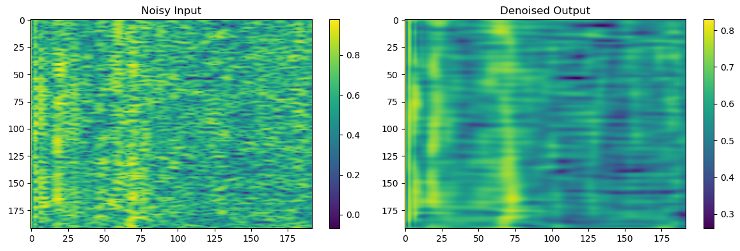
\includegraphics[width=\textwidth]{img/ch4/denoise/irfan.png}
%     \caption{Result of denoising with Input = Output using the Irfan architecture.}
% \end{figure}

\subsection{Masking-based techniques}

Masking-based denoising techniques focus on generating binary masks that highlight regions of interest, such as narrowband events, in the spectrogram \cite{zhou_self-noise_2023}. These masks can then serve as input features for classification models. It is a more extreme denoising method.

However, the primary roadblock with this method is that we do not have any ground truth data. We want ground truth masks of narrowband events; such datasets are not publically available due to the incredible amount of time needed to create these. Hence, we have two options: we label these ourselves, manually, or we try and approximate such labels using a masking algorithm from another domain of science.

The second roadblock is that our baseline inputs are too low resolution to accurately mark narrowband events.

\subsubsection{Verifying our models work}

Test that our four models work using the dataset presented in the original U-Net paper.

\subsubsection{Manual masking}

\paragraph{Labelling process}

Using MATLAB's Image Labeler tool, over 500 binary masks were manually created to annotate narrowband events. This process, while time-intensive, provided ground truth masks for evaluating automated masking methods.

\begin{figure}[htbp]
    \centering
    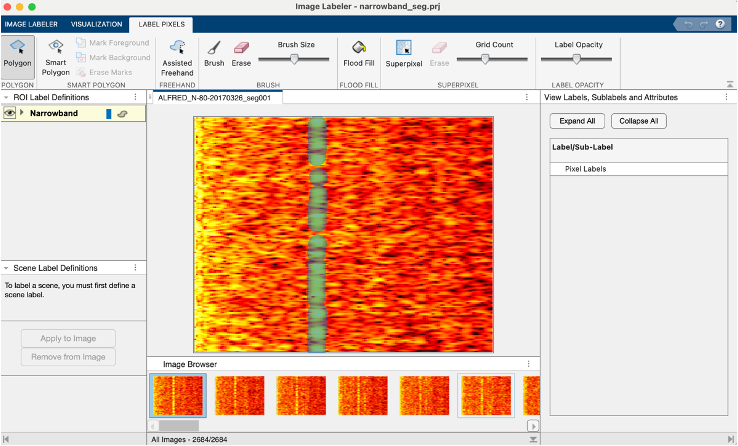
\includegraphics[width=0.8\textwidth]{img/ch4/denoise/matlab_image_labeller.png}
    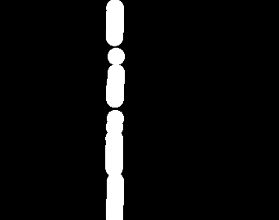
\includegraphics[width=0.7\textwidth]{img/ch4/denoise/binary_mask_ex.png}
    \caption{An example of a manually created binary mask of narrowband events using MATLAB Image Labeler. The top image shows the labeling process, while the bottom image shows the binary mask output.}
    \label{fig:manual-masks}
\end{figure}

\paragraph{Masking results}

Include diagrams here.

\paragraph{Classification results}

Feed the masks into CNN-LSTM and report the classification accuracy.

\subsubsection{Automated masking}

The HIDE \& SEEK algorithm was explored as a potential method for approximating narrowband event masks without manual labeling. 


